%! TeX program = lualatex
\documentclass[a4paper,11pt]{article} 
% packages
\usepackage{fontspec}
\setmainfont{EB Garamond}
% for tironian et fallback
% % \directlua{luaotfload.add_fallback
% % ("emojifallback",
% %      {"Noto Serif:mode=harf"}
% % )}
% % \setmainfont{EB Garamond}[RawFeature={fallback=emojifallback}]

\setmonofont[Scale=MatchLowercase]{Deja Vu Sans Mono}
\usepackage[a4paper,left=2cm,right=2cm,top=\dimexpr15mm+1.5\baselineskip,bottom=2cm]{geometry}
\setlength{\parindent}{0pt}

\usepackage{fancyhdr}       % Headers and footers 
\fancyhead[R]{\normalfont \leftmark}
\fancyhead[L]{}
\pagestyle{fancy}

\usepackage{microtype}      % Slightly tweak font spacing for aesthetics
\usepackage[english]{babel} % Language hyphenation and typographical rules
\usepackage[final, colorlinks = true, urlcolor = blue, linkcolor = black]{hyperref} 
\usepackage{changepage}     % adjust margins on the fly

\usepackage{minted}
\usepackage{xcolor}

\usepackage{pgfplots}
\pgfplotsset{width=\textwidth,compat=1.9}

\usepackage{caption}
\newenvironment{code}{\captionsetup{type=listing}}{}

\usepackage[yyyymmdd]{datetime}
\renewcommand{\dateseparator}{-}

\usepackage{titlesec}

\begin{document}
\begin{titlepage}
    \begin{center}
        \hrule
        \vspace*{0.6cm}
        \huge \textbf{CT3531}
        \vspace*{0.6cm}
        \hrule
        \LARGE
       \vspace{0.5cm}
        NETWORK \& DATA COMMUNICATIONS II
       \vspace{0.5cm}
       \hrule
            
       \vfill
       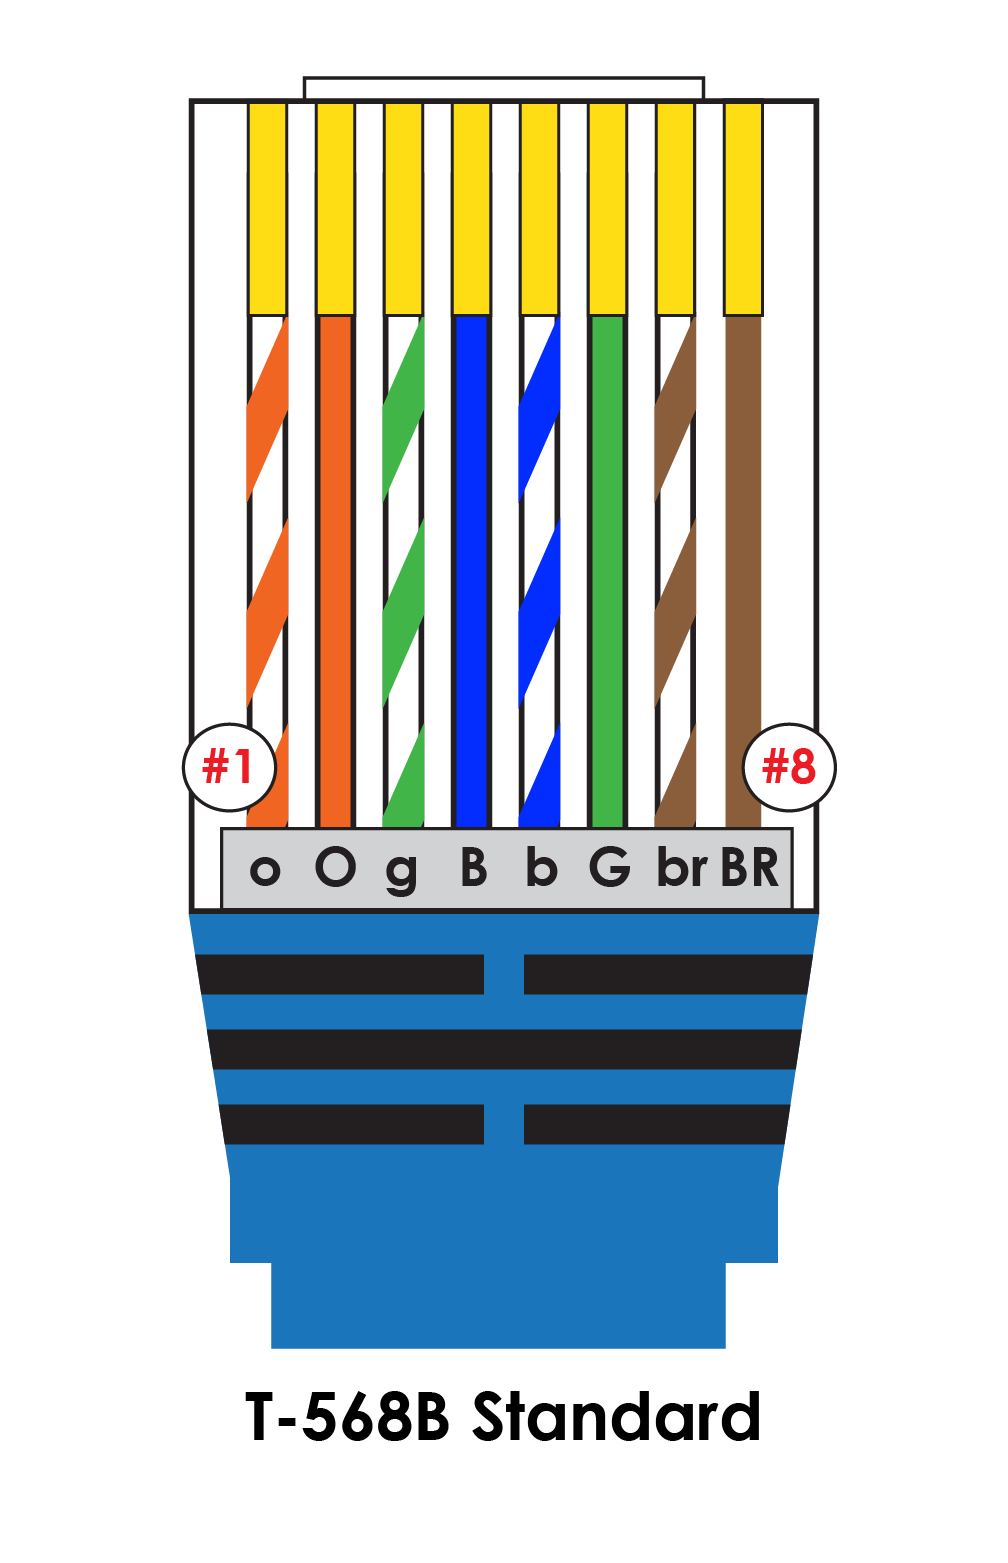
\includegraphics[width=0.6\textwidth]{images/commnet-systems-inc.png}
        \vfill

        \Large
       \vspace{0.5cm}
       \hrule
       \vspace{0.5cm}
       \textbf{Andreas Ó hAoḋa}
       % \vspace{0.5cm}
       % \hrule
       % \vspace{0.5cm}
            
       \normalsize
       University of Galway

       \today

       \vspace{0.5cm}
       \hrule
    \end{center}
\end{titlepage}

\pagenumbering{roman}
\newpage
\tableofcontents
\newpage
\setcounter{page}{1}
\pagenumbering{arabic}

\section{Introduction}
\subsection{Network Classification}
\begin{figure}[h]
    \centering
    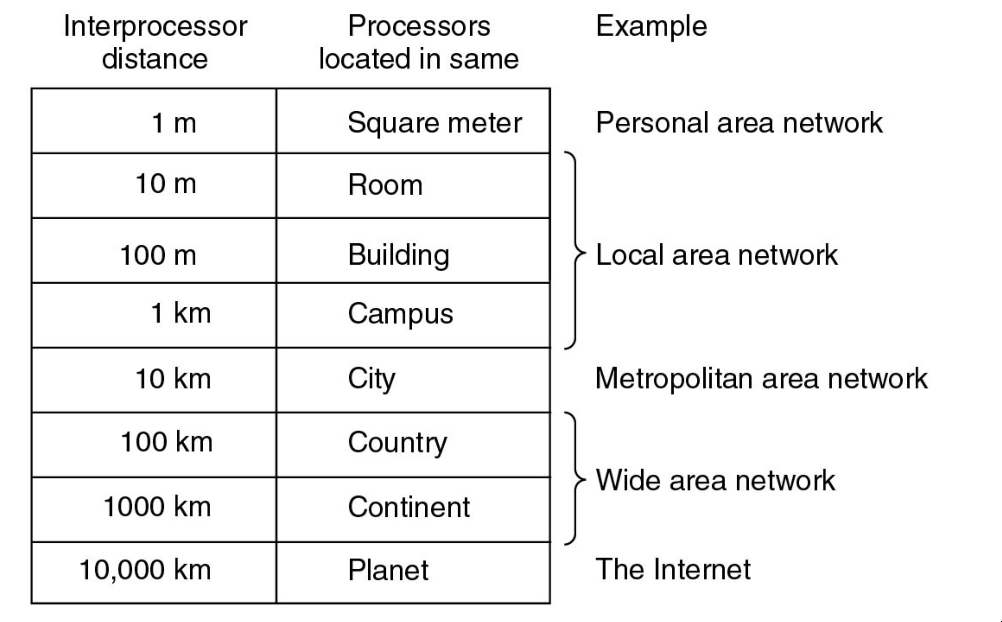
\includegraphics[width=0.7\textwidth]{./images/classification_of_interconnected_processors_by_scale.png}
    \caption{Classification of Interconnected Processors by Scale}
\end{figure}

\subsection{Reference Models}
The \textbf{Open Systems Interconnect (OSI) Reference Model}  is a network architecture based on a proposal developed by ISO 
to standardise the protocols used in various layers.
\begin{figure}[h]
    \centering
    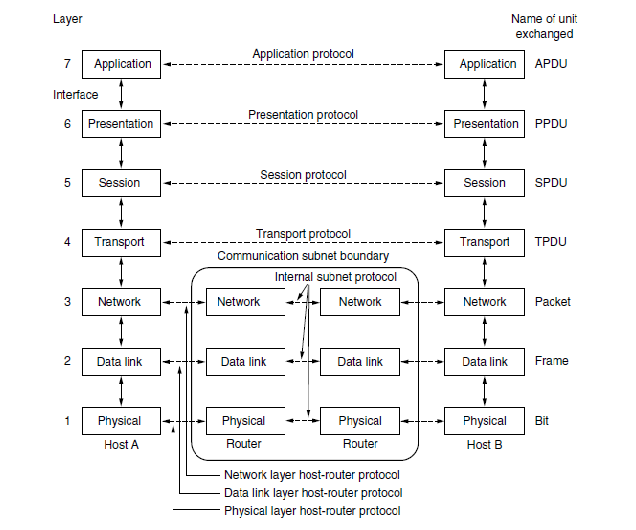
\includegraphics[width=0.7\textwidth]{./images/osireferencemodel.png}
    \caption{OSI Reference Model}
\end{figure}

The \textbf{TCP/IP Reference Model} is the model used by the Internet, a packet-switching network of networks based on a 
connectionless internetwork layer.
\begin{figure}[h]
    \centering
    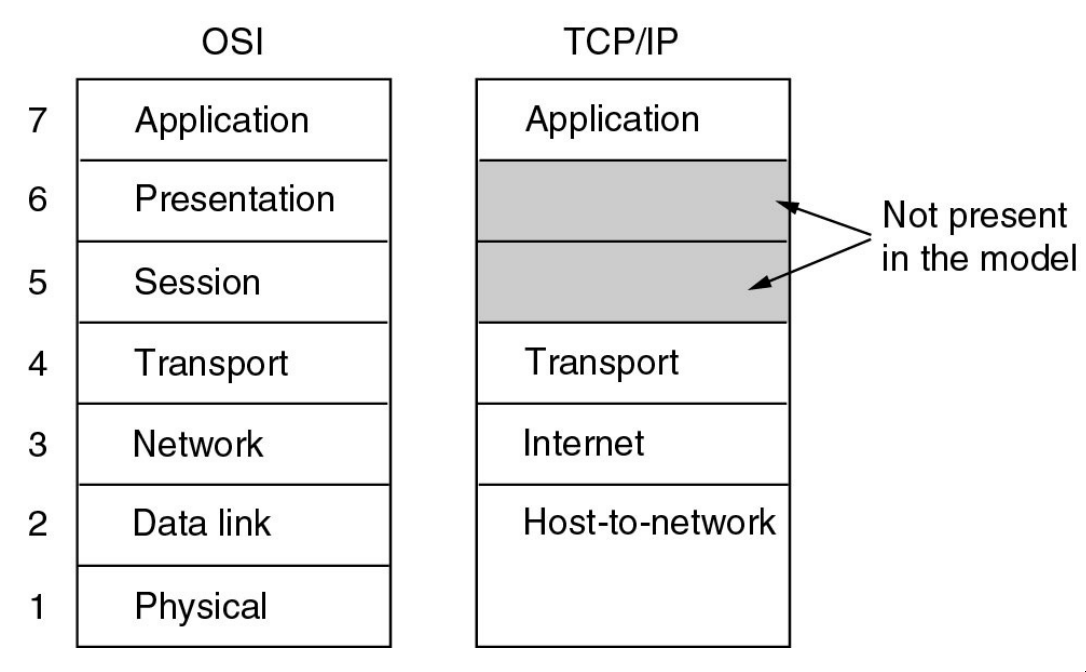
\includegraphics[width=0.7\textwidth]{./images/tcpipreferencemodel.png}
    \caption{OSI Reference Model}
\end{figure}

\subsection{DNS Name Space}
The Internet is divided into over 200 Top-Level Domains (TLDs). 
Each domain is divided into sub-domains, which are further partitioned, etc. 
All domains can be represented by a tree: The leaves of the tree represent domains that have no sub-domains (but contain
machines).
A leaf domain may contain a single host or represent a company and contain thousands of hosts.
Top-Level Domains could be generic and country domains. 
\\\\ 
One DNS server could theoretically service all requests, but in practice would be overloaded. 
To solve this, the \textbf{DNS name space} is divided into non-overlapping zones. 
Each zone contains some part of the tree \& name servers holding zone information. 
A zone would have a primary DNS which gets information from the disk, and one or more secondary DNS to get information from 
the primary DNS.

\subsection{Fibre Cables}
\begin{figure}[h]
    \centering
    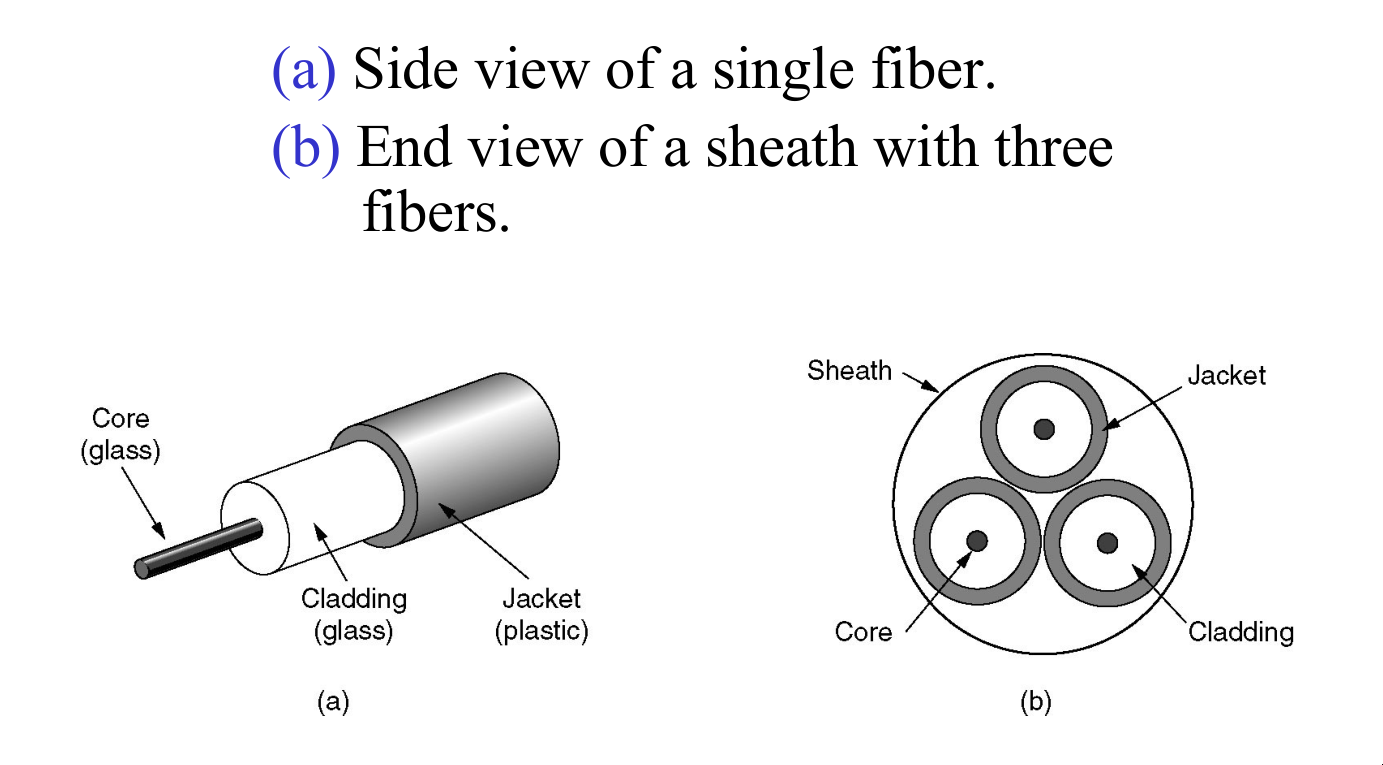
\includegraphics[width=0.7\textwidth]{./images/fibrecables.png}
    \caption{Fibre Cables}
\end{figure}

Optical networking \& Dense Wavelength-Division Multiplexing (DWDM) is rapidly bringing down the cost of networking, and 
further progress ``seems assured''.
Butter's ``Law'' states that the amount of data coming out of an optical fibre doubles every nine months. 
Thus, the cost of transmitting a bit over an optical network halves every nine months.

\section{Virtual LANs}
\subsection{Introduction}
\textbf{VLANs} logically segment switched networks based on the functions, project teams, or applications of the organisation 
regardless of the physical location or connections to the network. 
All workstations \& servers used by a particular workgroup share the same VLAN, regardless of the physical connection or location. 
\\\\ 
Broadcast traffic in LANs is sent to all devices on the LAN, but this can become a problem in large LANs. 
The traditional solution is to interconnect LANs by IP routers.
However, LAN membership of a host is tied to the local switch. 
\begin{figure}[H]
    \centering
    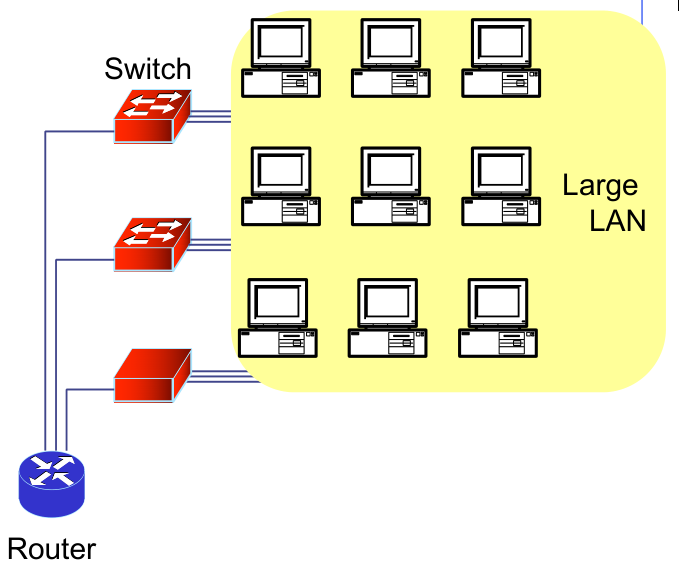
\includegraphics[width=0.5\textwidth]{./images/interconnected_lans.png}
    \caption{LANs Interconnected by IP Routers}
\end{figure}
A better solution is VLANs. 
VLANs separate the broadcast domain from the location of the hosts. 
This is used to partition large LANs.
VLANs are interconnected by IP routers. 
You can run a separate spanning tree in each VLAN.
\begin{figure}[H]
    \centering
    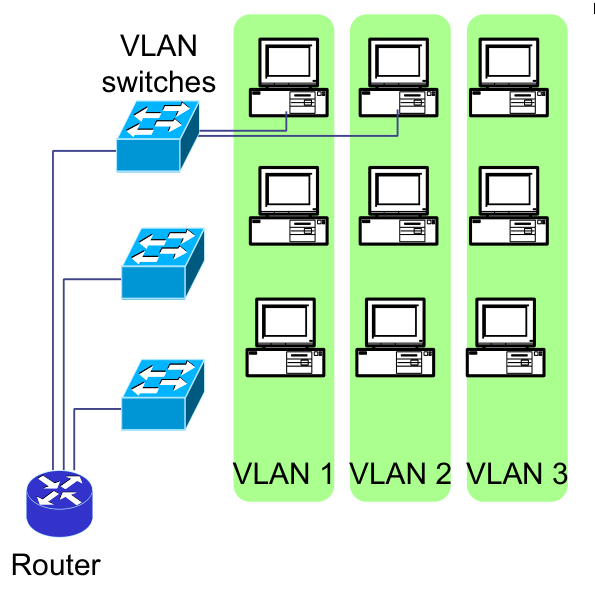
\includegraphics[width=0.5\textwidth]{./images/vlan.png}
    \caption{VLANs: The Better Solution}
\end{figure}

VLANs function by logically segmenting the network into different broadcast domains so that packets are only switched between 
ports that are designated for the same VLAN. 
Routers in VLAN topologies provide broadcast filtering, security, \& traffic flow management. 
VLANs address scalability, security, \& network management. 
Switches may not bridge any traffic between VLANs, as this would violate the integrity of the VLAN broadcast domain. 
Traffic should only be routed between VLANs.

\subsection{Broadcast Domains with VLANs \& Routers}
A VLAN is a broadcast domain created by one or more switches. 
A switch creates a broadcast domain, and VLANs help to manage broadcast domains. 
VLANs can be defined on pot groups, users, or protocols. 
LAN switches \& network management software provide a mechanism to create VLANs. 
\\\\ 
Layer 3 routing allows the router to send packets to the three different broadcast domains in this example. 
\begin{figure}[H]
    \centering
    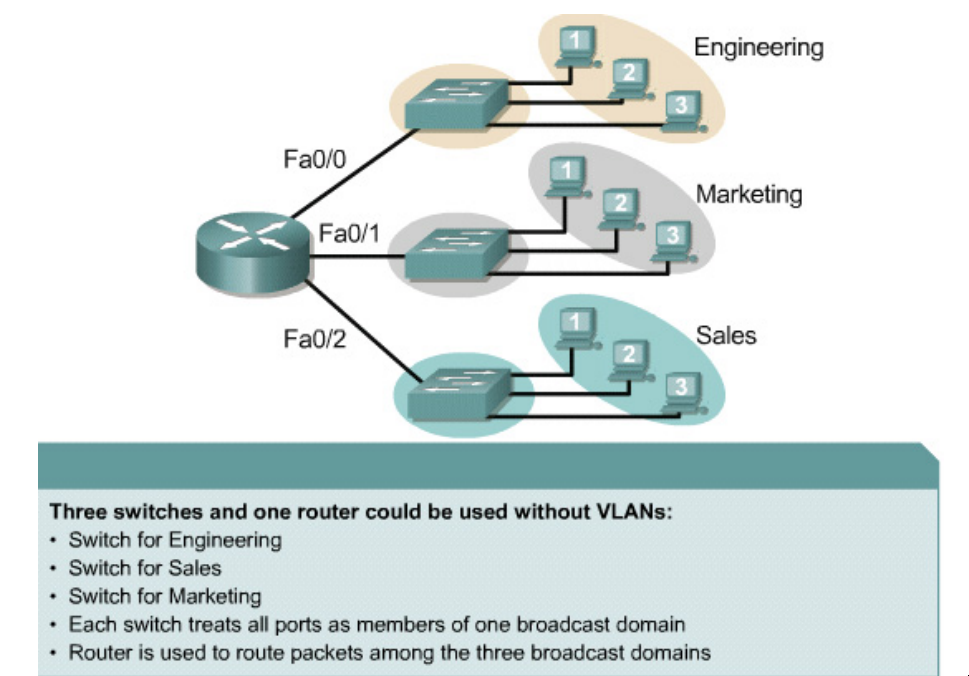
\includegraphics[width=0.8\textwidth]{./images/layer3_vlan.png}
    \caption{Broadcast Domains with VLANs \& Routers}
\end{figure}

Implementing VLANs on a switch causes the following to occur:
\begin{itemize}
    \item   The switch maintains a separate bridging table for each VLAN. 
    \item   If the frame comes in on a port in VLAN 1, the switch searches the bridging table for VLAN 1. 
    \item   When the frame is received, the switch adds the source address to the bridging table if it is currently 
            unknown.
    \item   The destination is checked so that a forwarding decision can be made. 
    \item   For learning \& forwarding, the search is made against the address table for that VLAN only.
\end{itemize}

\subsection{VLAN Operation}
Each switch port could be assigned to a different VLAN. 
Ports assigned to the same VLAN share broadcasts. 
Ports that do not belong to that VLAN do not share these broadcasts. 
\begin{figure}[H]
    \centering
    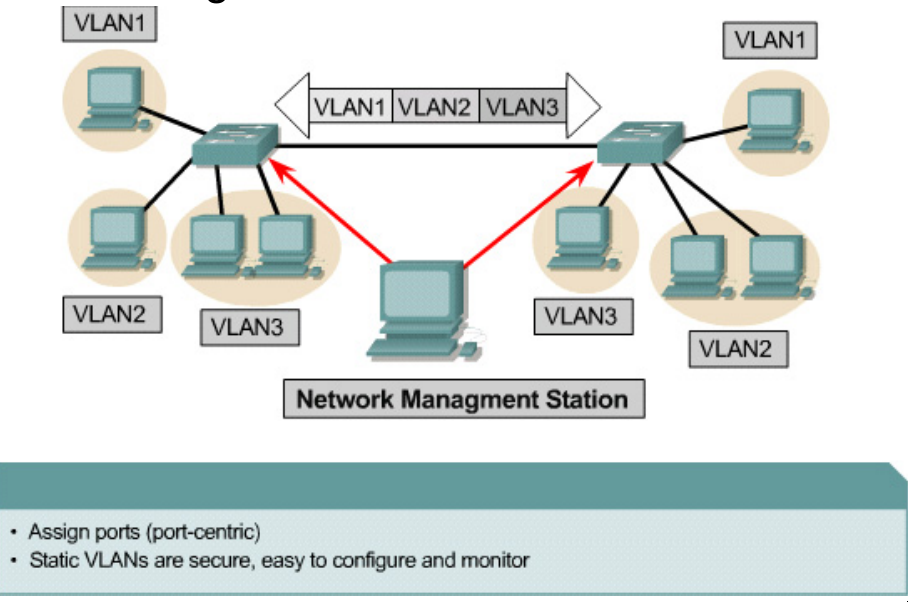
\includegraphics[width=0.8\textwidth]{./images/vlan_operation.png}
    \caption{VLAN Operation}
\end{figure}

Users attached to the same shared segment share the bandwidth of that segment. 
Each additional user attached to the shared medium means less bandwidth and deterioration of network performance. 
VLANs offer more bandwidth to users than a shared network. 
The default VLAN for every port in the switch is the \textbf{management VLAN}.
The management VLAN is always VLAN 1 and cannot be deleted. 
All other ports on the switch may be re-assigned to alternate VLANs.
\\\\ 
Dynamic VLANs allow for membership based on the MAC address of the device connected to the switch port. 
As a device enters the network, it queries a database within the switch for a VLAN membership. 
\begin{figure}[H]
    \centering
    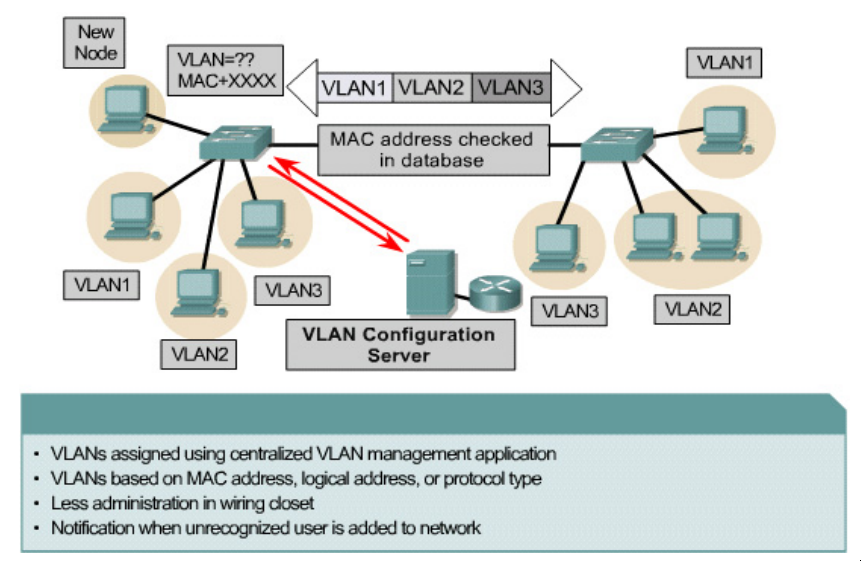
\includegraphics[width=0.8\textwidth]{./images/vlan_operation1.png}
    \caption{VLAN Operation}
\end{figure}

In port-based or port-centric VLAN membership, the port is assigned to a specific VLAN membership, independent of the user 
or the system attached to the port. 
All users of the same port must be in the same VLAN.
\\\\ 
Network administrators are responsible for configuring VLANs both statically \& dynamically. 
Configuring VLANs \textbf{statically} involves the network administrators configuring it port-by-port. 
Each port is associate with a specific VLAN. 
The network administrator is responsible for keying in the mappings between the ports \& VLANs. 
Configuring VLANs \textbf{dynamically} means that the ports are able to dynamically work out their VLAN configuration. 
This uses a software database of MAC addresses to VLAN mappings which the network administrator must set up first.

\subsection{Benefits of VLANs}
The key benefit of VLANs is that they permit the network administrator to organise the LAN \emph{logically} instead of 
physically. 

\subsection{VLAN Types}
There are three basic VLAN memberships for determining \& controlling how a packet gets assigned:
\begin{itemize}
    \item   Port-based. 
    \item   MAC address-based.
    \item   Protocol-based.
\end{itemize}

The frame headers are encapsulated or modified to reflect a VLAN ID before the frame is sent over the link between switches. 
The frame header is changed back to the original format before forwarding to the destination device.
\\\\ 
The number of VLANs in a switch vary depending on several factors, including:
\begin{itemize}
    \item   Traffic patterns. 
    \item   Types of applications. 
    \item   Network management needs. 
    \item   Group commonality.
\end{itemize}

An important consideration in defining the size of the switch and the number of VLANs is the \textbf{IP addressing scheme}.
Because a one-to-one correspondence between VLANs \& IP subnets is strongly recommended, there can be no more than 254 
devices in any one VLAN. 
It is further recommended that VLANs should not extend outside of the Layer 2 domain of the distribution switch.

\subsubsection{Membership by Port}
\begin{figure}[H]
    \centering
    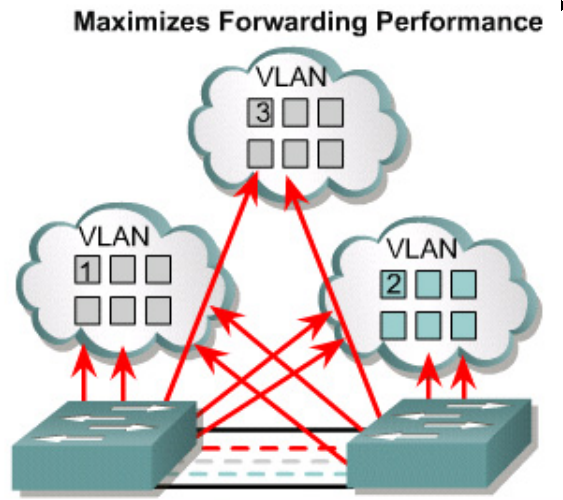
\includegraphics[width=0.5\textwidth]{./images/membership_by_port.png}
    \caption{Membership by Port}
\end{figure}

\begin{itemize}
    \item   User assigned by port association. 
    \item   Requires no lookup if done in ASICs. 
    \item   Easily administered via GUIs. 
    \item   Packets do not ``leak'' into other domains. 
    \item   Easily controlled across network.
\end{itemize}

\subsubsection{Membership by MAC-Addresses}
\begin{figure}[H]
    \centering
    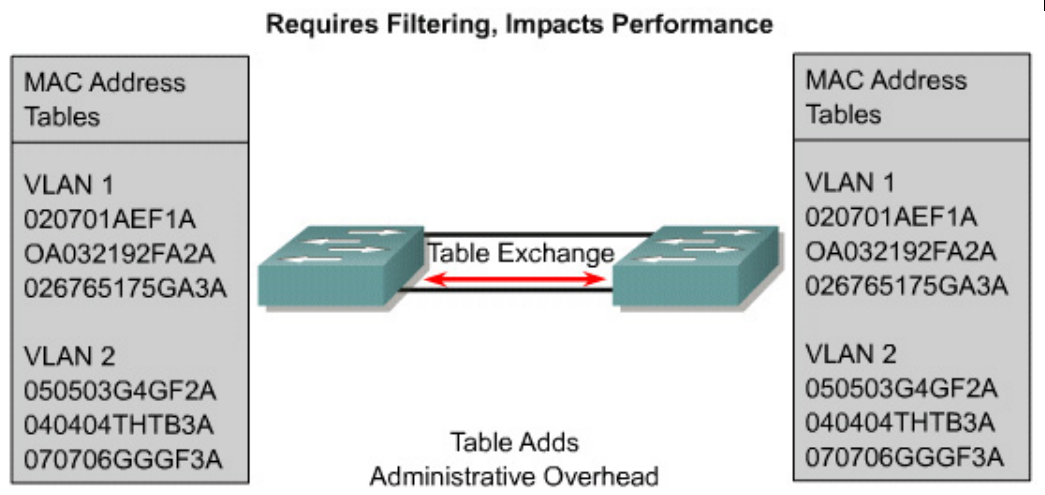
\includegraphics[width=0.7\textwidth]{./images/membership_by_mac.png}
    \caption{Membership by MAC-Address}
\end{figure}

\begin{itemize}
    \item   User assigned based on MAC addresses. 
    \item   Offers flexibility, yet adds overhead. 
    \item   Impacts performance, scalability, \& administration. 
    \item   Offers similar process for higher layers.
\end{itemize}

\subsection{VLANs Across Multiple Switches}
If VLANs span multiple switches, then the traffic between the switches belong to different VLANs.
Switches need to be able to demultiplex traffic from different VLANs.
\textbf{VLAN tags} are used for this purpose.

\subsubsection{IEEE 802.1Q: VLAN Tagging}
For VLAN traffic between LAN switches, add a tag to Ethernet frames that identifies the LAN. 
The tag can be transparent to endsystems, by stripping off the VLAN tag.
\begin{figure}[H]
    \centering
    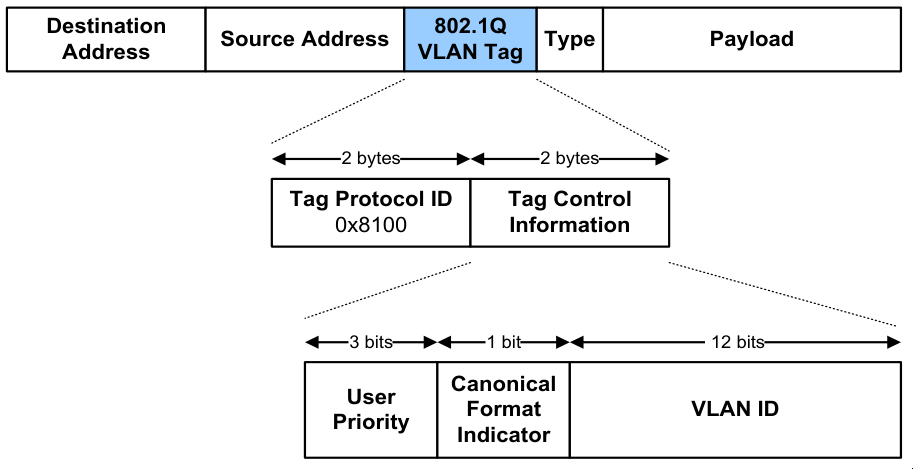
\includegraphics[width=0.8\textwidth]{./images/vlan_tagging.png}
    \caption{VLAN Tagging}
\end{figure}

The 802.1Q Tag Fields are:
\begin{itemize}
    \item   \textbf{Tag Protocol Identifier:} Value \verb|0x8100| identifies 802.1Q tag. 
    \item   \textbf{User Priority:} Can be used by the sender to prioritise different types of traffic (e.g., voice, data).
            0 is the lowest priority.
    \item   \textbf{Canonical Format Indicator:} Used for compatibility between different types of MAC protocols.
    \item   \textbf{VLAN Identifier (VID):} Specifies the VLAN (1-4094). \verb|0x000| indicates that the frame does not 
            belong to a VLAN. \verb|0xfff| is reserved.
\end{itemize}

The normal operation of VLAN tags is as follows:
\begin{itemize}
    \item   Sender sends frame.
    \item   First switch adds tag.
    \item   Last switch removes tag.
\end{itemize}

\subsection{Spanning-Tree Protocols}
Bridges \& switches use the \textbf{Spanning-Tree Protocol (STP)} to avoid loops.
Bridges (switches) running STP participate with other bridges in the election of a single bridge as the \textbf{Root Bridge}.
They calculate the distance of the shortest path to the Root Bridge and choose a port (known as the \textbf{Root Port}) 
that provides the shortest path to the Root Bridge. 
For each LAN segment, they elect a \textbf{Designated Bridge} and a \textbf{Designated Port} on that bridge. 
The Designated Port is a port on the LAN segment that is closed to the Root Bridge. 
All ports on the Root Bridge are Designated Ports).
The bridge ports to be included in the spanning tree are selected. 
The ports selected are the Root Ports \& Designated Ports. 
These ports forward traffic, while the other ports block traffic.
\begin{figure}[H]
    \centering
    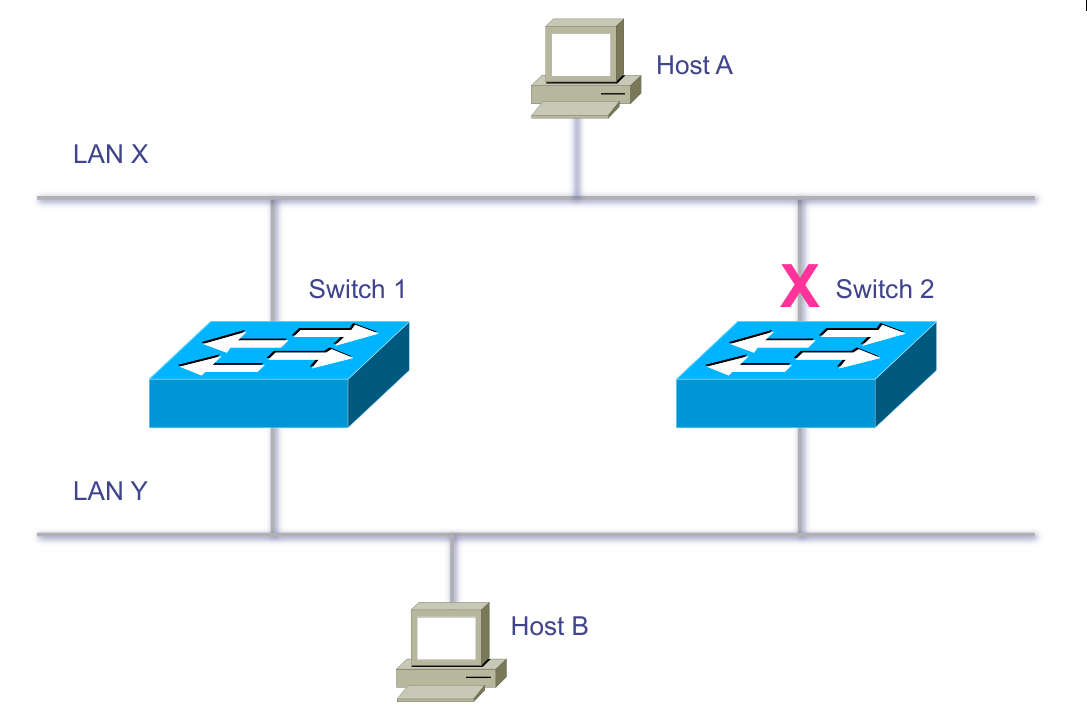
\includegraphics[width=0.6\textwidth]{./images/stp.png}
    \caption{Spanning-Tree Protocols}
\end{figure}

\begin{figure}[H]
    \centering
    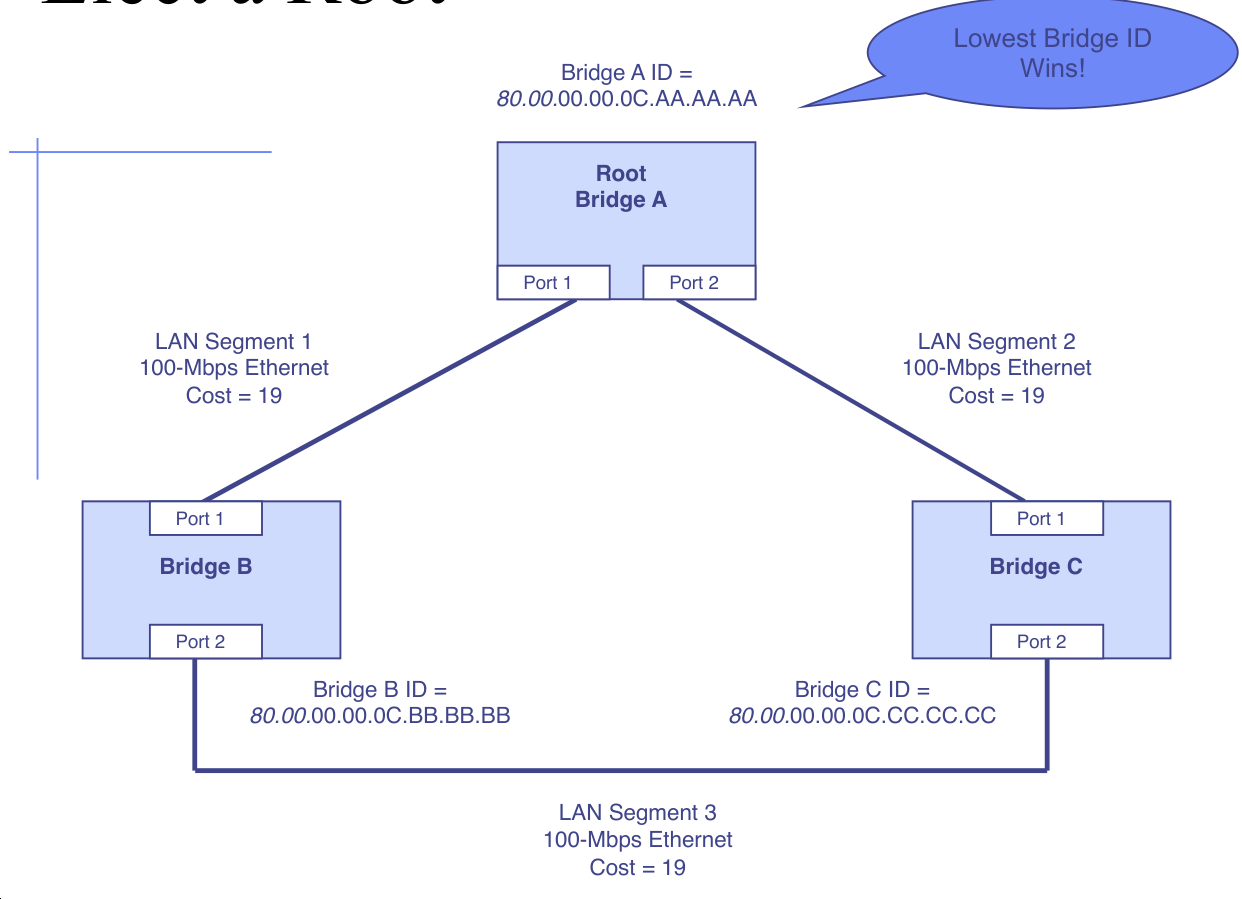
\includegraphics[width=0.8\textwidth]{./images/electing_root.png}
    \caption{Electing a Root Bridge}
\end{figure}

\begin{figure}[H]
    \centering
    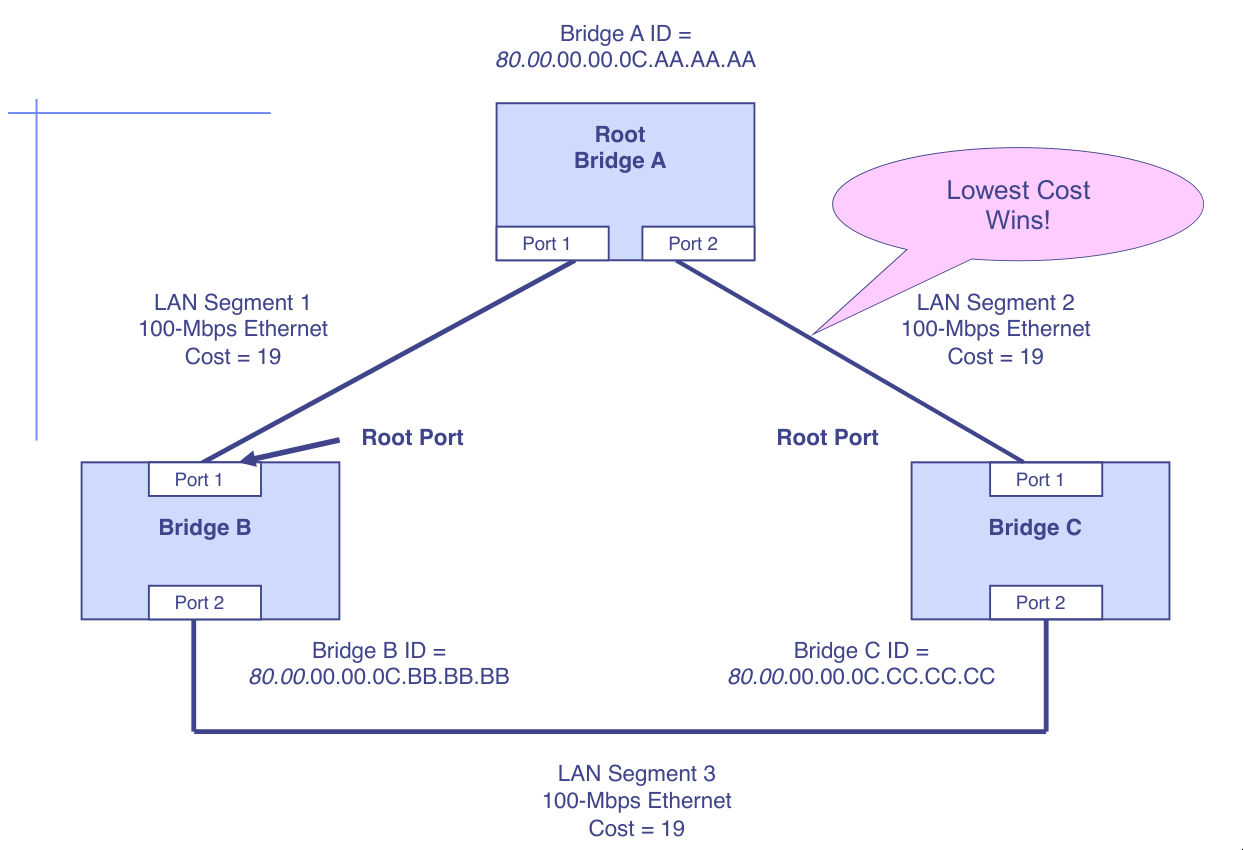
\includegraphics[width=0.8\textwidth]{./images/determine_root_ports.png}
    \caption{Determining Root Ports}
\end{figure}

\begin{figure}[H]
    \centering
    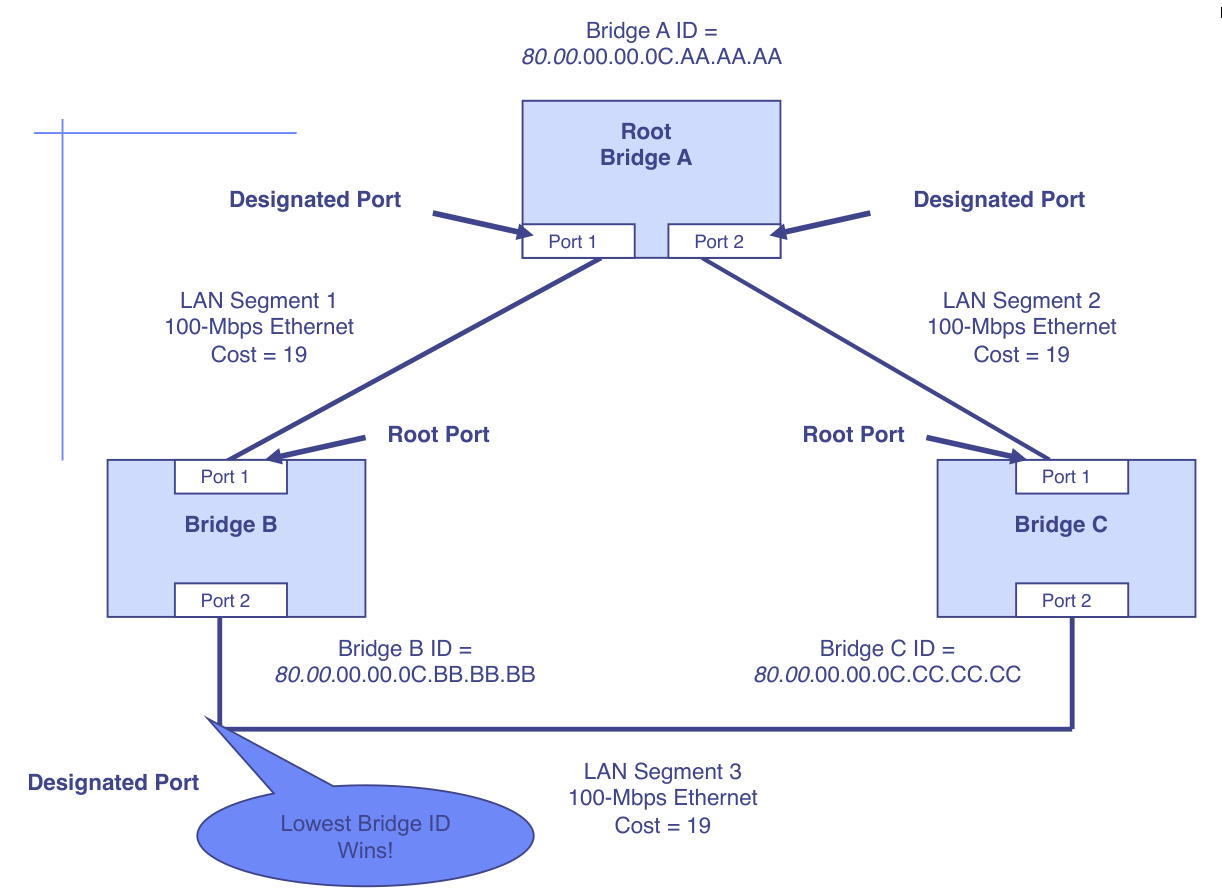
\includegraphics[width=0.8\textwidth]{./images/determine_designated_ports.png}
    \caption{Determining Designated Ports}
\end{figure}

\begin{figure}[H]
    \centering
    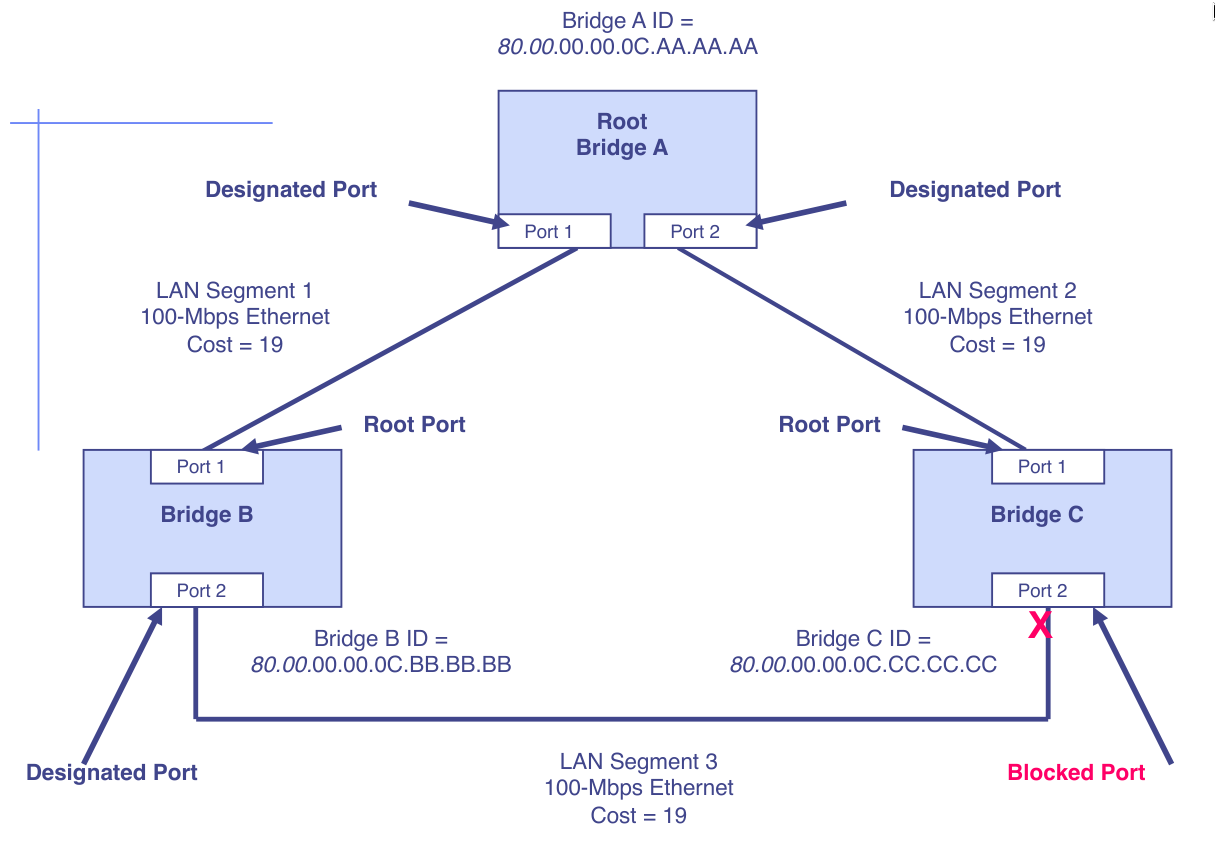
\includegraphics[width=0.8\textwidth]{./images/prune_into_tree.png}
    \caption{Pruning the Topology into a Tree}
\end{figure}

\begin{figure}[H]
    \centering
    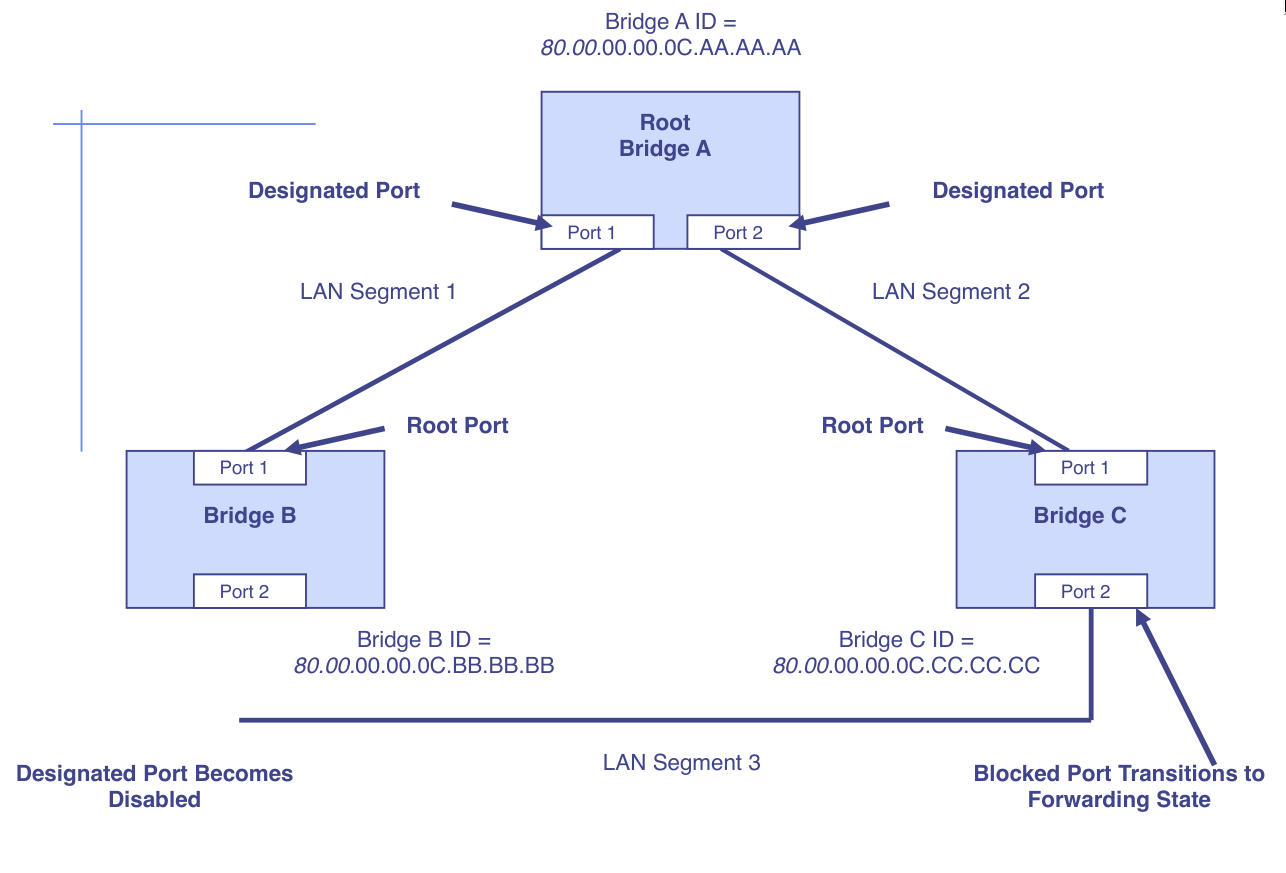
\includegraphics[width=0.8\textwidth]{./images/react_to_changes.png}
    \caption{Reacting to Changes}
\end{figure}

\subsubsection{Scaling the STP}
\begin{itemize}
    \item   Keep the switched network small; it shouldn't span more than 7 switches.
    \item   Use BDPU skew detection on Cisco switches. 
    \item   Use IEEE 802.1w: Provides rapid reconfiguration of the spanning tree. Also known as RSTP.
\end{itemize}

\section{Addressing \& Naming}
\subsection{Guidelines for Addressing \& Naming}
\begin{itemize}
    \item   Use a structured model for addressing \& naming.
            This makes it easier to:
            \begin{itemize}
                \item   Read network maps.
                \item   Operate network management software.
                \item   Recognise devices in protocol analyser traces.
                \item   Meet goals for usability.
                \item   Design filters on firewalls \& routers.
                \item   Implement route summarisation.
            \end{itemize}
    \item   Assign addresses \& names hierarchically.
    \item   Decide in advance if you will use:
            \begin{itemize}
                \item   Central or distributed authority for addressing \& naming.
                \item   Public or private addressing.
                \item   Static or dynamic addressing \& naming.
            \end{itemize}
\end{itemize}

\subsection{Public \& Private IP Addresses}
Public IP addresses are managed by the Internet Assigned Number Authority (IANA). 
Users are assigned IP addresses by Internet Service Providers (ISPs).
ISPs obtain allocations of IP addresses from their appropriate Regional Internet Registry (RIR).
\begin{itemize}
    \item   American Registry for Internet Numbers (ARIN) serves North America and parts of the Caribbean. 
    \item   RIPE Network Coordination Centre (RIPE NCC) serves Europe, the Middle East, and Central Asia. 
    \item   Asia-Pacific Network Information Centre (APNIC) serves Asia and the Pacific region. 
    \item   Latin American and Caribbean Internet Addresses Registry (LACNIC) serves Latin America and parts of the
            Caribbean. 
    \item   African Network Information Centre (AfriNIC) serves Africa. 
\end{itemize}

The private IP address ranges are:
\begin{itemize}
    \item   \verb|10.0.0.0| -- \verb|10.255.255.255|.
    \item   \verb|172.16.0.0| -- \verb|172.31.255.255|.
    \item   \verb|192.168.0.0| -- \verb|192.168.255.255|.
\end{itemize}

\subsection{Criteria for Using Static vs Dynamic Addressing}
\begin{itemize}
    \item   The number of end systems.
    \item   The likelihood of needing to re-number.
    \item   The need for high availability.
    \item   Security requirements.
    \item   The importance of tracking addresses.
    \item   Whether end systems need additional information (DHCP can provide more than just an address).
\end{itemize}

\subsection{The Anatomy of an IP Address}
An IP address consists of a \textbf{Prefix} \& a \textbf{Host}.
\begin{figure}[H]
    \centering
    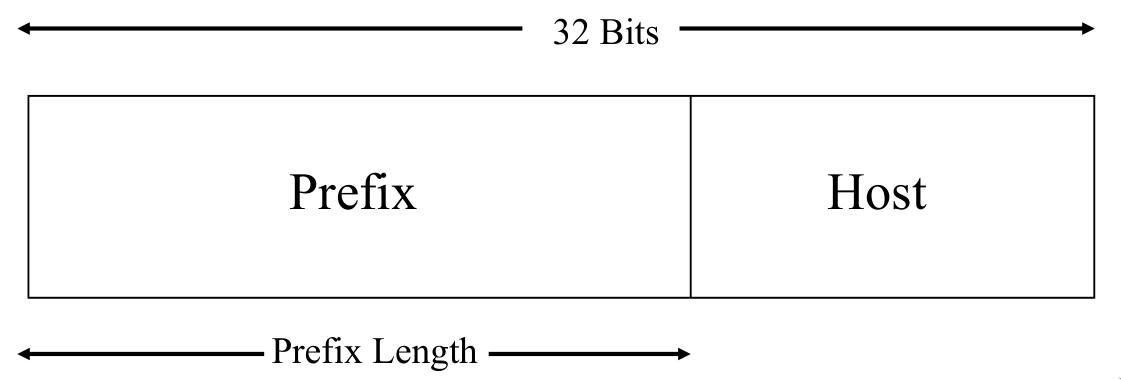
\includegraphics[width=0.8\textwidth]{./images/ipaddr_anatomy.png}
    \caption{The Two Parts of an IP Address}
\end{figure}

An IP address is accompanied by an indication of the prefix length, either a \textbf{subnet mask} or the \verb|/<length>|
notation, e.g. \verb|192.168.10.1 255.255.255.0| or \verb|192.168.10.1/24|.
The subnet mask is 32 bits long and specifies which part of an IP address is the network/subnet field and which part is the 
host field. 
The network/subnet portion of the mask is all \verb|1|s in binary.
The host portion of the mask is all \verb|0|s in binary.
The binary expression must be converted back to dotted-decimal notation for entering into configurations.
Alternatively, you can use the \textbf{slash notation}, e.g. \verb|/24|, which specifies the number of \verb|1|s.

\subsection{Designing Networks with Subnets}
\subsubsection{Addresses to Avoid when Subnetting}
\begin{itemize}
    \item   A node address of all \verb|1|s (broadcast).
    \item   A node address of all \verb|0|s (network).
    \item   A subnet address of all \verb|1|s (all subnets).
    \item   A subnet address of all \verb|0|s (confusing).
            CISCO IOS configuration permits a subnet address of all zeros with the \verb|ip subnet-zero| command.
\end{itemize}

\section{Dynamic Routing Algorithms}
\subsection{Routing Algorithms}
A router can be seen as a device that contains two processes:
\begin{itemize}
    \item   The first process is the \textbf{forwarding process} which handles each packet as it arrives, 
            looking up for the outgoing  line to use for it.
    \item   The other process is responsible for filling in \& updating the routing tables; this is where the 
            \textbf{routing algorithm} comes into play.
\end{itemize}

Certain properties are desirable for a routing algorithm, such as correctness, simplicity, robustness, stability,
fairness, \& optimality.
Fairness \& optimality may sound obvious, but they are often contradictory goals:
suppose that there is enough traffic between $A$ \& $A'$, $B$ \& $B'$, $C$ \& $C'$ to saturate the horizontal 
links. 
To maximise the total flow, the $XX'$ traffic should be shut down completely.
Evidently, some sort of compromise between global efficiency \& fairness to individual connections is needed.

\subsubsection{The Optimality Principle}
If a router $J$ is on the optimal path from the router $I$ to the router $K$, then the optimal path from $J$ to 
$K$ follows the same route. 
A direct consequence of the optimality principle is that we can see that all optimal routes from all sources to 
a given destination form a tree rooted at the destination called a \textbf{sink tree};
the tree in the below figure is a sink tree for router $B$ in the subnet, where the metric is the number of hops. 
The goal of all routing algorithms is to discover \& use the sink tree for all routers.
\begin{figure}[H]
    \centering
    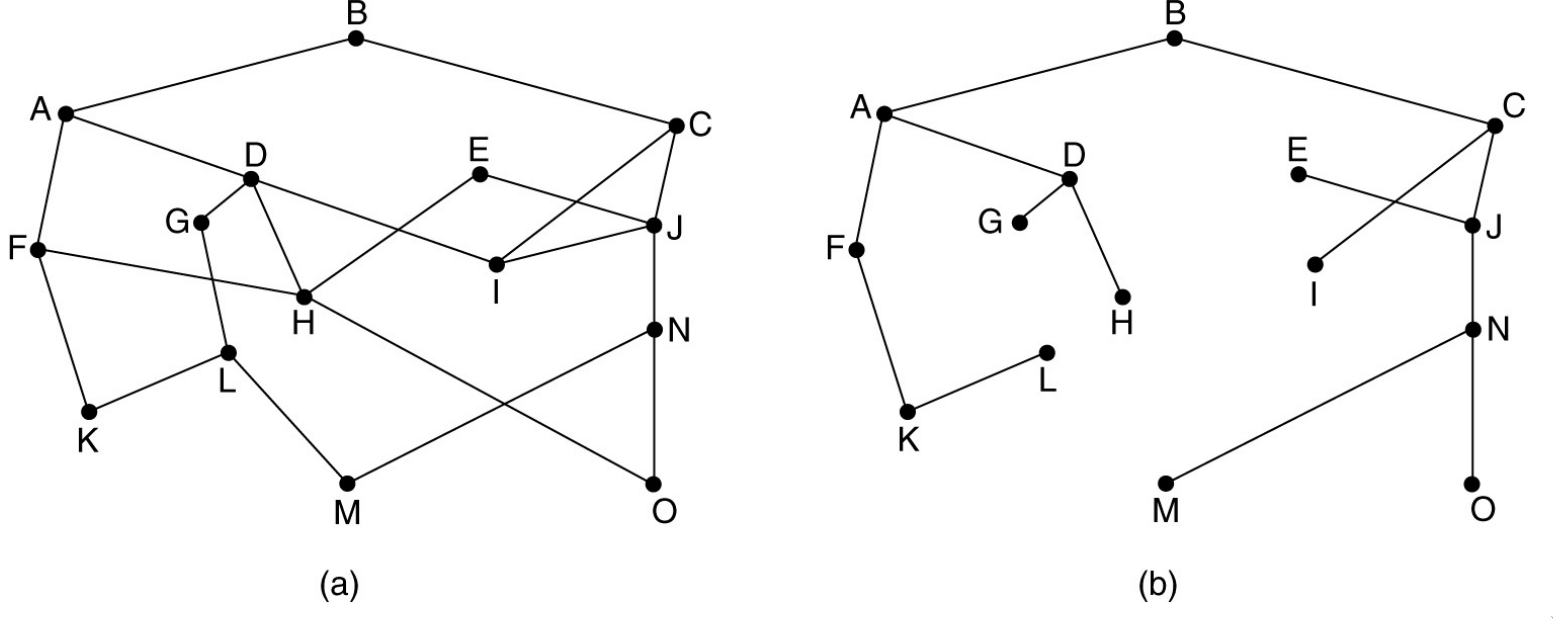
\includegraphics[width=0.8\textwidth]{./images/optimality_principle.png}
    \caption{Sink Trees}
\end{figure}

\subsection{Types of Routing Algorithms}
\textbf{Static (non-adaptive) routing algorithms} don't base their routing decisions on measurements or estimates
of the current traffic and/or topology.
The choice of the route to use from $I$ to $J$ is computed in advance (offline) and downloaded into the routers
at network boot time.
\\\\
\textbf{Dynamic (adaptive) routing algorithms} change their routing decisions to reflect changes in topology and
usually changes in traffic as well.
They differ how they get their information, e.g. locally, from the adjacent router, or from all routers, when 
they change the routes, or what metrics they use for optimisation, e.g. distance, number of hops, estimated 
transit time, etc.
Computer networks usually use dynamic routing algorithms, since that static ones don't take in calculus the 
network loads.

\subsubsection{Flooding Routing}
\textbf{Flooding} is a static algorithm in which every incoming packet is sent out on every outgoing line 
except the one that it arrived on. 
It generates a vast number of duplicate packets, and therefore some measures must be taken to dampen the process,
such as having a hop counter contained in the header (decremented by each router) with the packet being discarded
when the counter reaches 0 or keeping track of which packets have been flooded so that flooding again can be 
avoided.
\\\\ 
In \textbf{selective flooding}, the routers don't send every incoming packet out on every line, but only on those 
lines that are going in the approximate right direction.
\\\\
Flooding is not practical in most applications, but it does have some use in applications where tremendous 
robustness is highly desirable (e.g., military applications, where routers are deployed at once, radio networks, 
etc.). 
Flooding can also be used as a metric against which other routing algorithms can be compared.
Flooding always chooses the shortest path because it chooses every possible path in parallel.
Consequently, no other algorithm can produce a shorter delay (if we ignore the overhead...).

\subsection{Shortest Path Routing}
The idea of \textbf{shortest path routing} is to build a graph of the subnet, which each node of the graph
representing a router and each arc of the graph representing a communication line (link).
To choose a route between a given pair of routers, the algorithm needs to find the shortest path between them on 
the graph.
\begin{figure}[H]
    \centering
    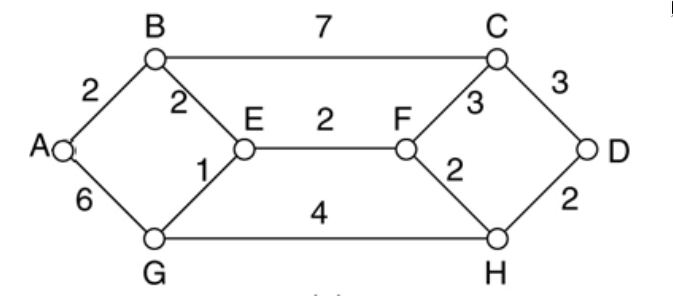
\includegraphics[width=0.5\textwidth]{./images/example_subnet_graph.png}
    \caption{Example Subnet Graph}
\end{figure}

Metrics for shortest path routing include:
\begin{itemize}
    \item   Number of hops: above, $ABC$ \& $ABE$ are 
            equally long.
    \item   Geographic distance: ABC is clearly much longer than ABE, assuming that the above diagram is to scale.
    \item   Other metrics: each arch could be labelled with the mean queuing \& transmission delay for some 
            standard test packet as determined by hourly test runs; with this graph labelling, the shortest 
            path is the fastest path rather than the path with the fewest hops or kilometers.
\end{itemize}

The labels on the arcs could be computed as a function of many factors: distance, average traffic, bandwidth, 
communication cost, mean queue length, measured delay, \& other factors.
By changing the criteria, the algorithm will then compute the shortest path according to the measuring criteria
or combination of criteria.

\subsubsection{Dijkstra's Algorithm for Computing the Shortest Path}
Each node is labeled with its distance from the source node along the best known path. 
Initially, no paths are known, so all nodes are labeled with $\infty$.
As the algorithm proceeds and paths are found, the label may change to reflect better paths.
A label may be either tentative or permanent; initially are labels are tentative. 
When it is discovered that a label represents the shortest possible path from the source to that node, it is made
permanent and never changed after that.
\begin{figure}[H]
    \centering
    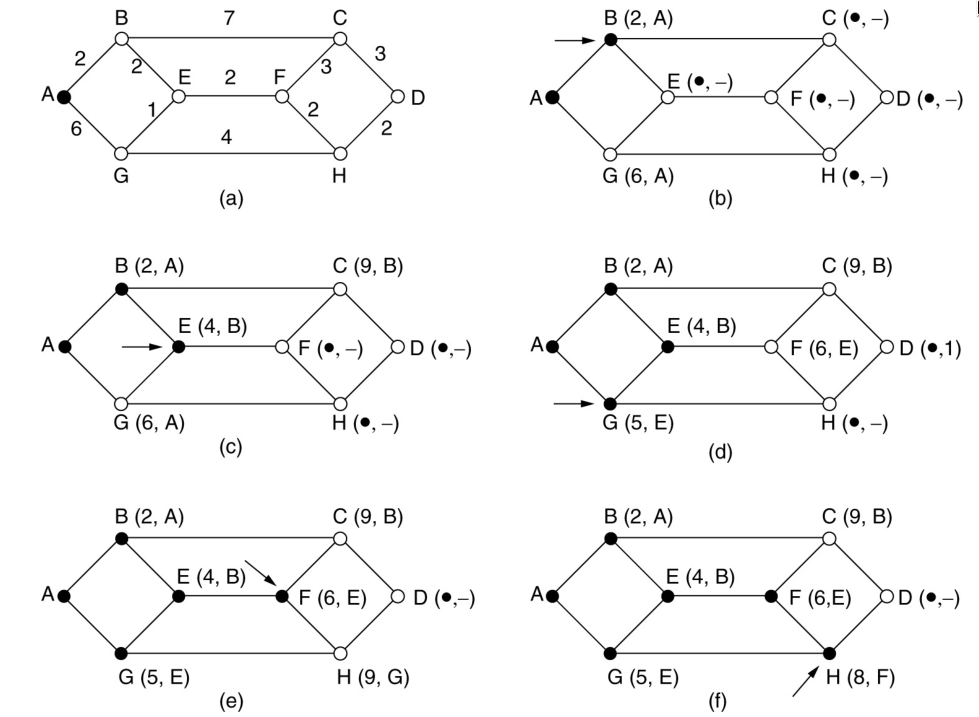
\includegraphics[width=0.8\textwidth]{./images/dijkstra.png}
    \caption{Dijkstra's Algorithm Example}
\end{figure}

\subsection{Distance Vector Routing}
\textbf{Distance Vector Routing} was used in ARPANET and is sometimes used in the Internet under the name
\textbf{RIP}.
Each router maintains a table (i.e., a vector) giving the best known distance to each destination and which line
to use to get there.
These tables are updated by exchanging information with the neighbours.
The routing table contains an entry for each router in the subnet.
This entry contains two parts:
\begin{itemize}
    \item   Preferred outgoing line to use for that destination.
    \item   The estimation of the time or distance to that destination (the used metric can be the number of hops,
            time delay in milliseconds, the total number of packets queued along that or something similar).
\end{itemize}

The router is assumed to know the distance to each of its neighbours:
\begin{itemize}
    \item   If the metric is hops, the distance is just hop.
    \item   If the metric is time, the router can measure it directly with special echo packets.
    \item   If it is queue length, the router examines each of its queues.
\end{itemize}

\begin{figure}[H]
    \centering
    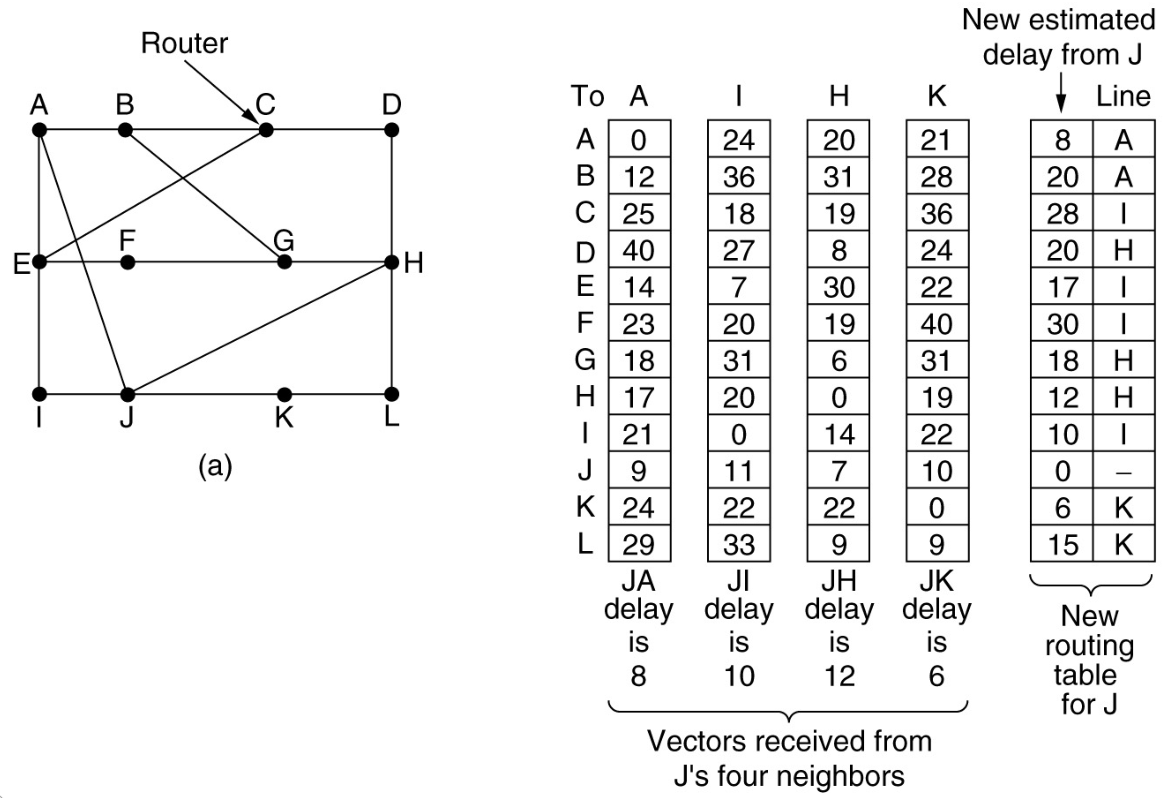
\includegraphics[width=0.8\textwidth]{./images/distance_vector_routing.png}
    \caption{Distance Vector Routing}
\end{figure}

\begin{enumerate}
    \item   $J$ measures the delays to its neighbours.
    \item   $J$ computes its new routes to router $G$:
            \begin{itemize}
                \item   It knows that it can get to $A$ in 8ms and $A$ claims to get to $G$ in 18ms, so $J$ knows
                        that it can count on packets with 26ms to $G$ if it routes the packets through $A$.
                \item   Similarly, it computes delays to $G$ via $I$ ($10 + 31$), via $H$ ($12+6$), \& via $K$ 
                        ($6+31$). 
                        The best of these values is 18 so it makes an entry in its routing table that the delay 
                        to $G$ is 18ms and the route to use is via $H$.
            \end{itemize}
    \item   The same calculation is performed to all other destinations.
\end{enumerate}

\subsection{Link State Routing}
Distance vector routing was replaced by link state routing for two reasons:
\begin{itemize}
    \item   Distance vector routing's delay metric is \textbf{queue length}; it didn't take in calculus the line 
            bandwidth.
    \item   The distance vector routing algorithm takes too long to converge.
\end{itemize}

Each router must do the following:
\begin{itemize}
    \item   Discover their neighbours and learn their net addresses.
    \item   Measure the delay or cost to each of their neighbours.
    \item   Construct a packet telling all it has just learned.
    \item   Send this packet to all the other routers.
    \item   Compute the shortest path to every other router.
\end{itemize}

\subsubsection{Distance Vector vs Link State Routing}
\begin{itemize}
    \item   With distance vector routing, each node has information only about the next hop.
    \item   Distance vector routing makes poor routing decisions if directions are not completely correct (e.g., 
            because a node is down).
            If parts of the directions are incorrect, the routing may be incorrect until the routing algorithms 
            have re-converged.
    \item   In link state routing, each node has a complete map of the topology.
    \item   If a node fails in link state routing, each node can calculate a new route. 
    \item   The main difficulty with link state routing is that all nodes need to have a consistent view of the 
            network.
\end{itemize}

\subsubsection{Basic Principles of Link State Routing}
\begin{enumerate}
    \item   Each router establishes a relationship called an \textbf{adjacency} with its neighbours.
    \item   Each router generates \textbf{Link State Advertisements (LSAs)} which are distributed to all routers.
            An LSA consists of a link ID, the state of the link, the cost, \& the neighbours of the link.
    \item   Each router maintains a database of all received LSAs called a \textbf{topological database} or 
            \textbf{link state database}, which describes the network as a graph with weighted edges.
    \item   Each router uses its link state database to run a shortest path algorithm (Dijkstra's algorithm) to 
            produce the shortest path to each network.
\end{enumerate}

\begin{figure}[H]
    \centering
    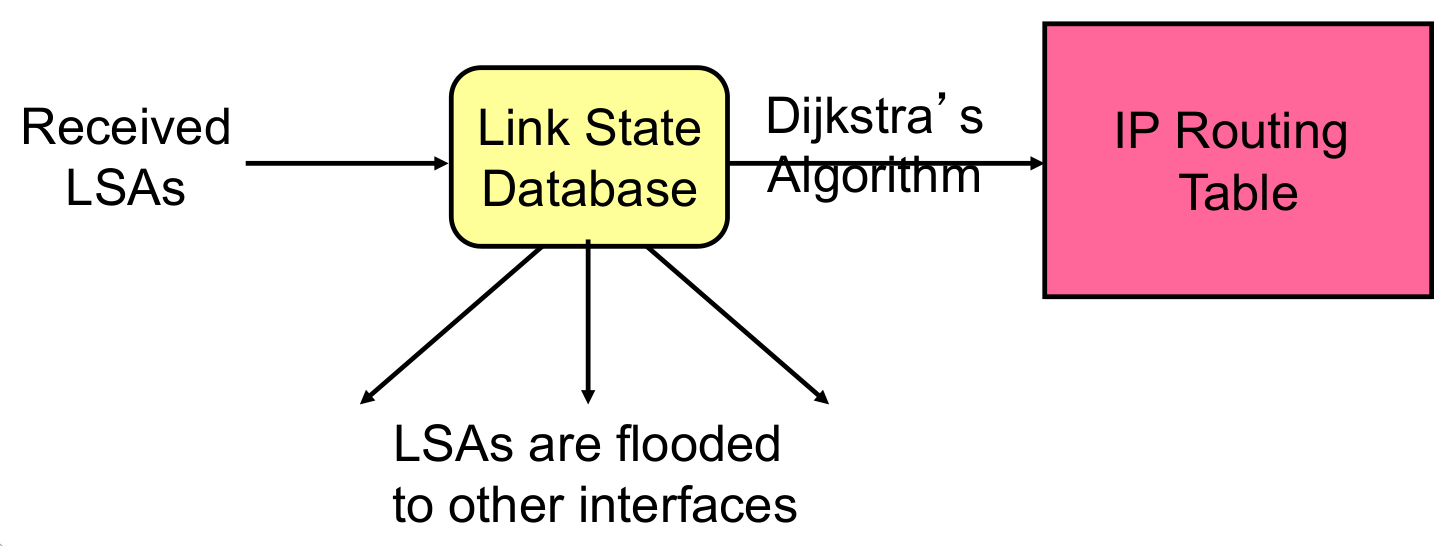
\includegraphics[width=0.8\textwidth]{./images/lsr_protocol.png}
    \caption{Operation of a Link State Routing Protocol}
\end{figure}

\subsection{OSPF}
The \textbf{OSPF (Open Shortest Path First)} routing protocol is the most important link state routing protocol on 
the Internet. 
The complexity of OSPF is significant.
Features of OSPF include:
\begin{itemize}
    \item   Provides authentication of routing messages.
    \item   Enables load balancing by allowing traffic to be split evenly across routes with equal cost.
    \item   Type-of-Service routing allows the setup of different routes dependent on the TOS field.
    \item   Supports subnetting.
    \item   Supports multicasting.
    \item   Allows hierarchical routing.
\end{itemize}

\begin{figure}[H]
    \centering
    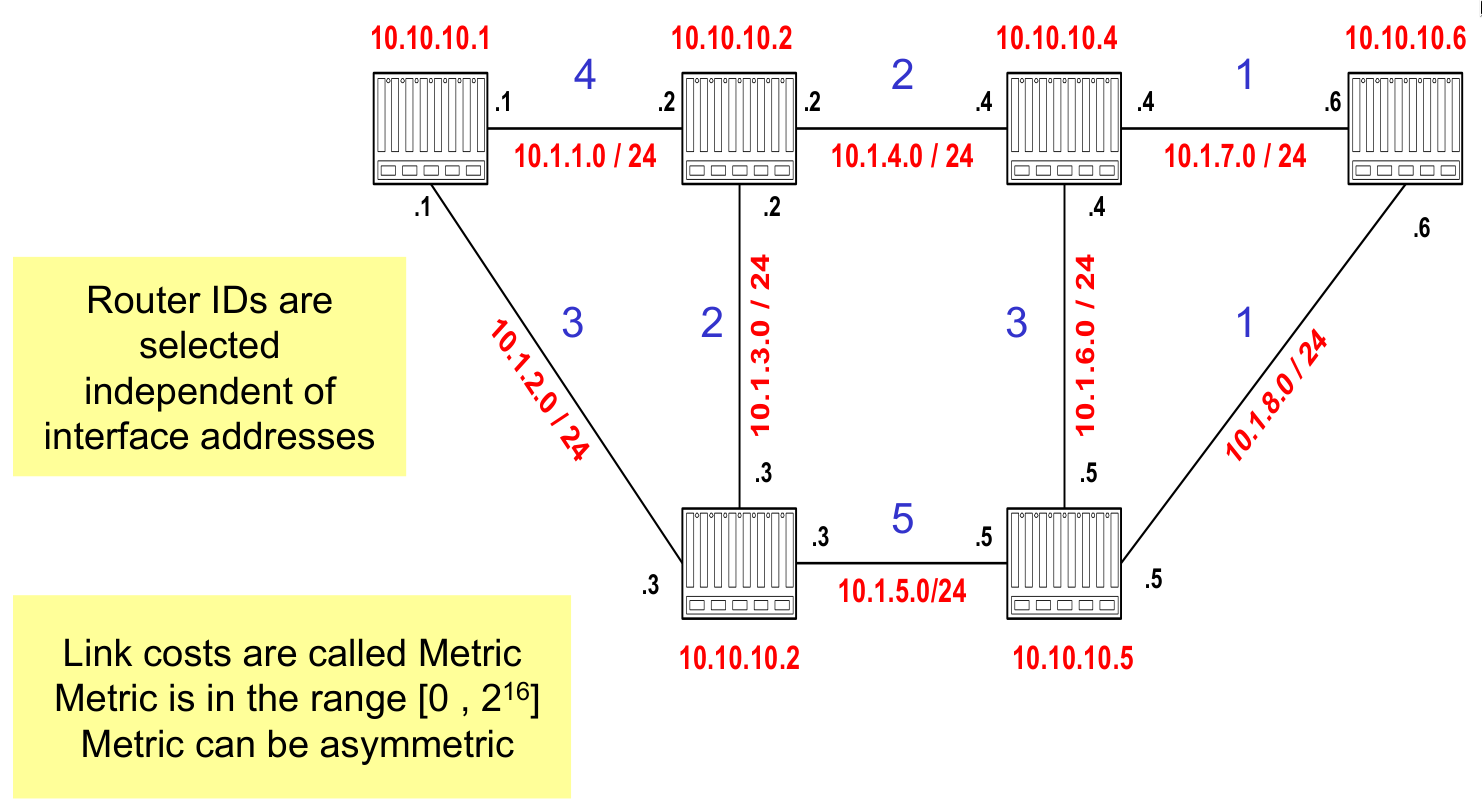
\includegraphics[width=0.8\textwidth]{./images/ospf_example.png}
    \caption{OSPF in an Example Network}
\end{figure}

\subsubsection{Link State Advertisement (LSA)}
Each router sends its LSA to all routers in the network using a method called \textbf{reliable flooding}.
The LSA of router  \verb|10.10.10.1| from the previous example is as follows:
\begin{itemize}
    \item   Link State ID: \verb|10.10.10.1| = Router ID.
    \item   Advertising Router: \verb|10.10.10.1| = Router ID.
    \item   Number of links: 3 = 2 links plus the router itself.
    \item   Description of Link 1: Link ID = \verb|10.1.1.1|, Metric = 4.
    \item   Description of Link 2: Link ID = \verb|10.1.2.1|, Metric = 3.
    \item   Description of Link 3: Link ID = \verb|10.10.10.1|, Metric = 0.
\end{itemize}

Each router has a database which contains the LSAs from all the other routers.
The collection of all LSAs is called the \textbf{link-state database}. 
Each router has an identical link-state database; this is very useful for debugging, as every router has a complete 
description of the network.
If neighbouring routers discover each other for the first time, they will exchange their link-state databases.
The link-state databases are synchronised using \textbf{reliable flooding}.

\subsection{OSPF Packet Format}
\begin{figure}[H]
    \centering
    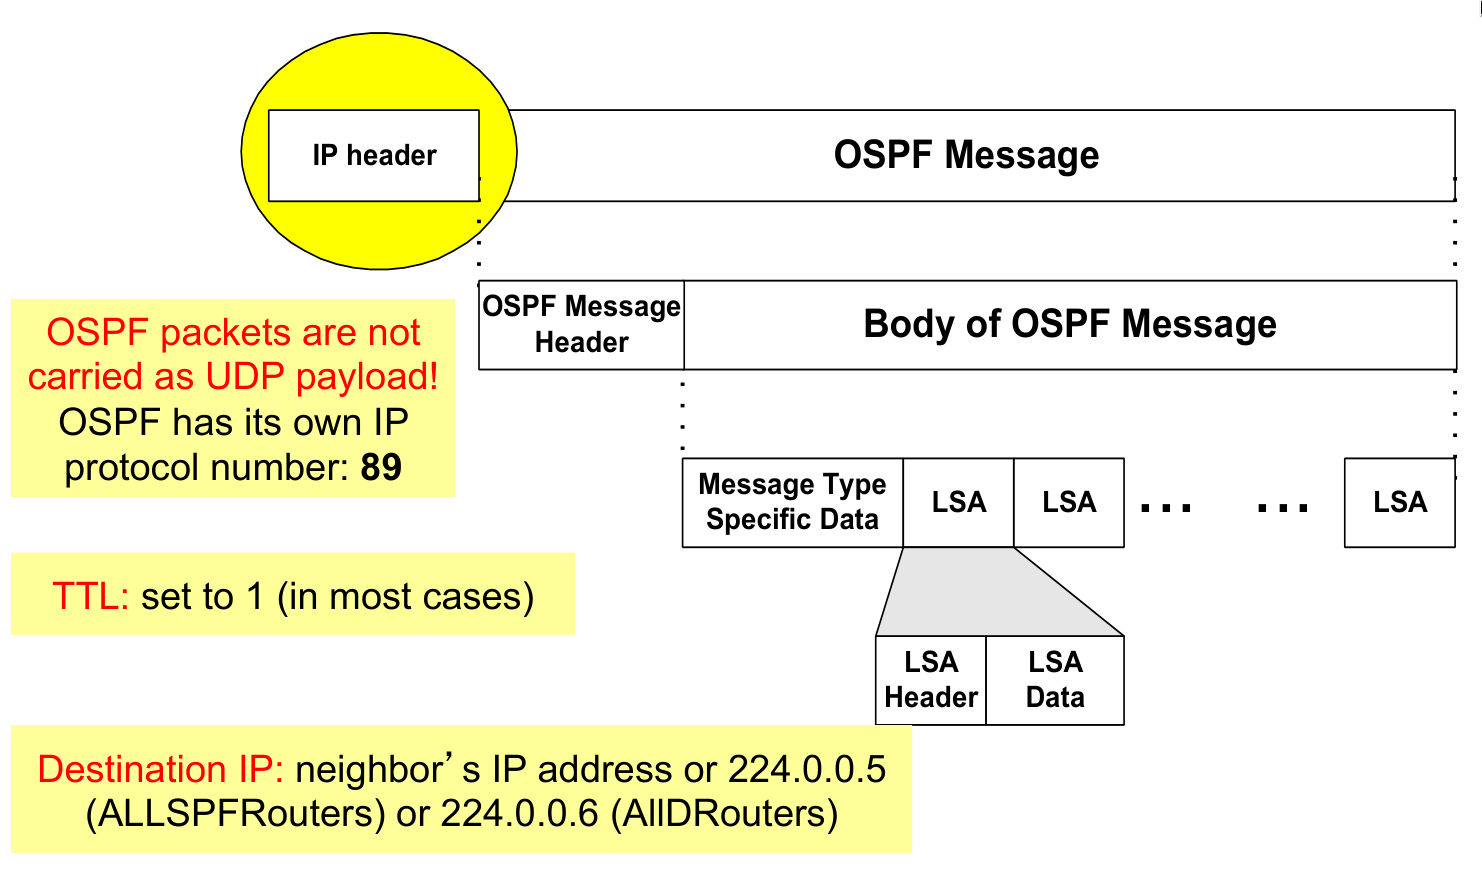
\includegraphics[width=0.8\textwidth]{./images/ospf_packet_format.png}
    \caption{OSPF Packet Format 1}
\end{figure}
\begin{figure}[H]
    \centering
    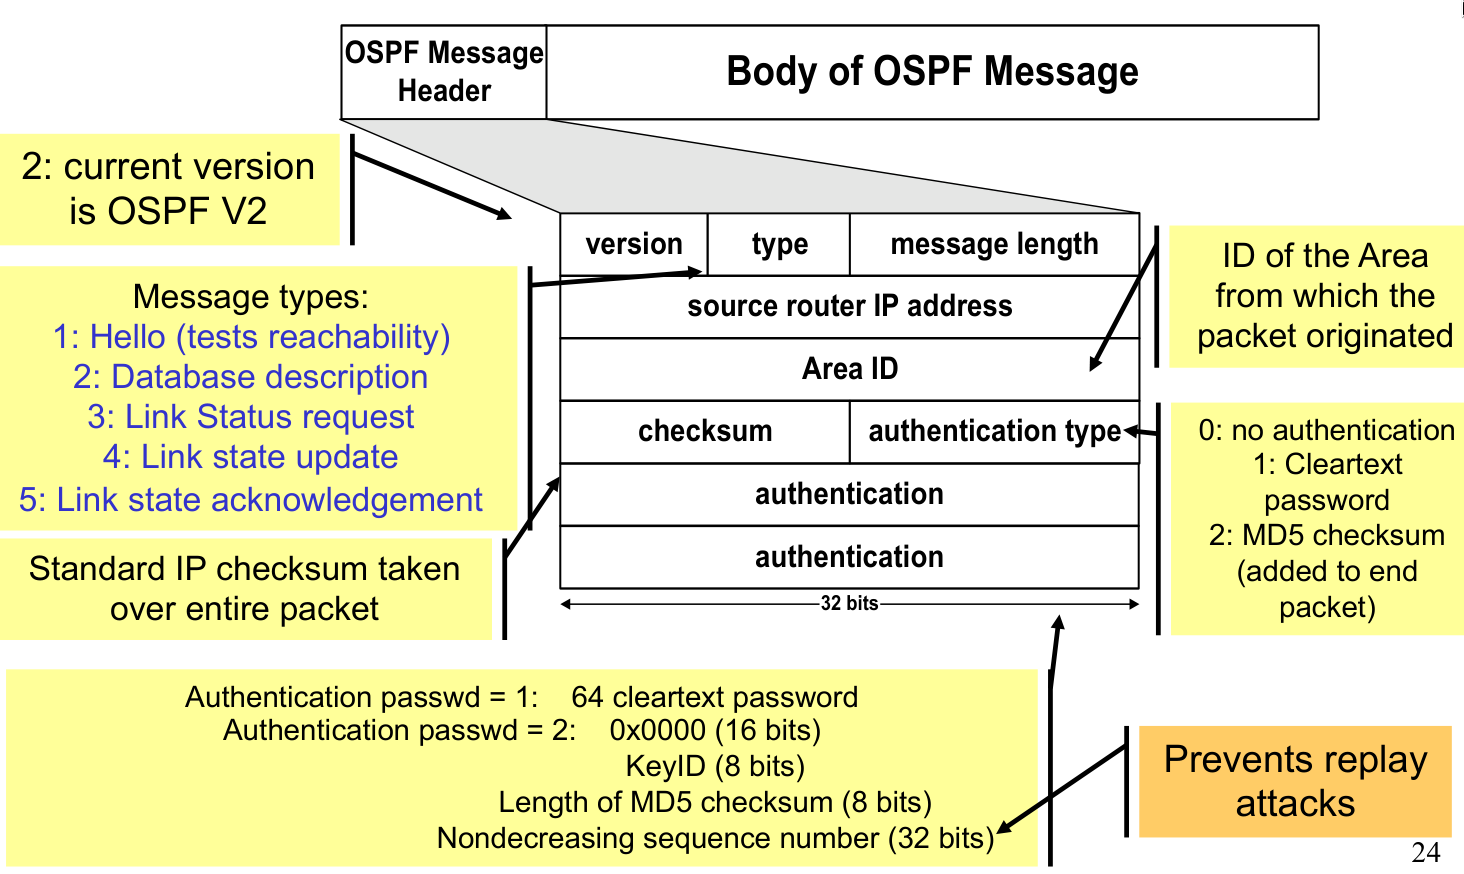
\includegraphics[width=0.8\textwidth]{./images/ospf_packet_format2.png}
    \caption{OSPF Packet Format 2}
\end{figure}
\begin{figure}[H]
    \centering
    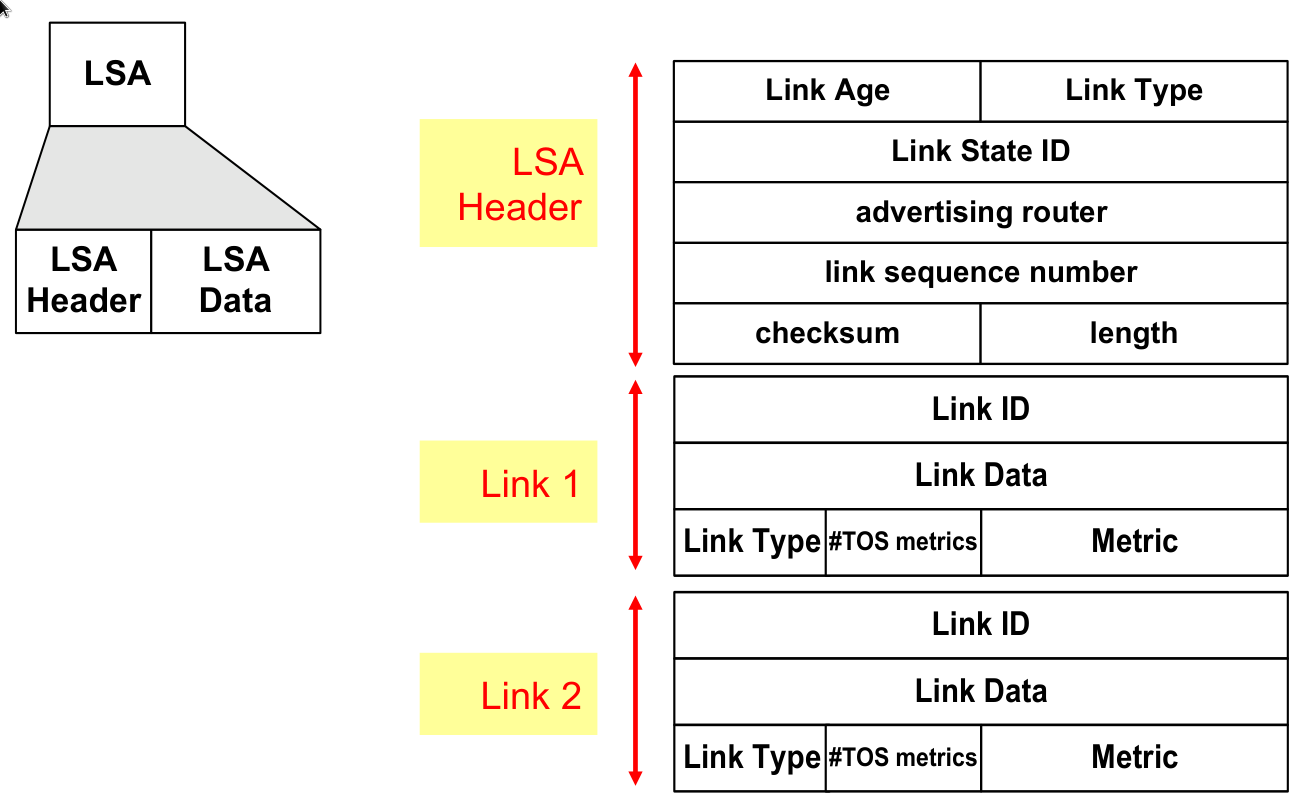
\includegraphics[width=0.8\textwidth]{./images/ospf_lsa_format.png}
    \caption{OSPF LSA Format}
\end{figure}

\subsection{Discovery of Neighbours}
The routers multicast \textbf{OSPF Hello packets} on all OSPF-enable interfaces. 
If two routers share a link, they can become neighbours and establish adjacency.
\begin{figure}[H]
    \centering
    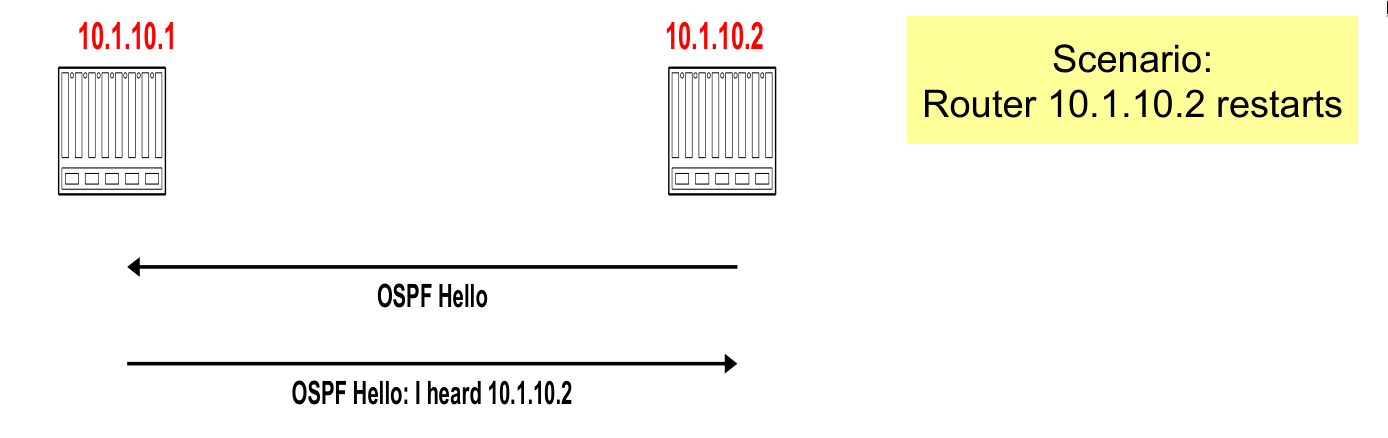
\includegraphics[width=0.8\textwidth]{./images/neighbour_discovery.png}
    \caption{Discovery of Neighbours}
\end{figure}

\begin{figure}[H]
    \centering
    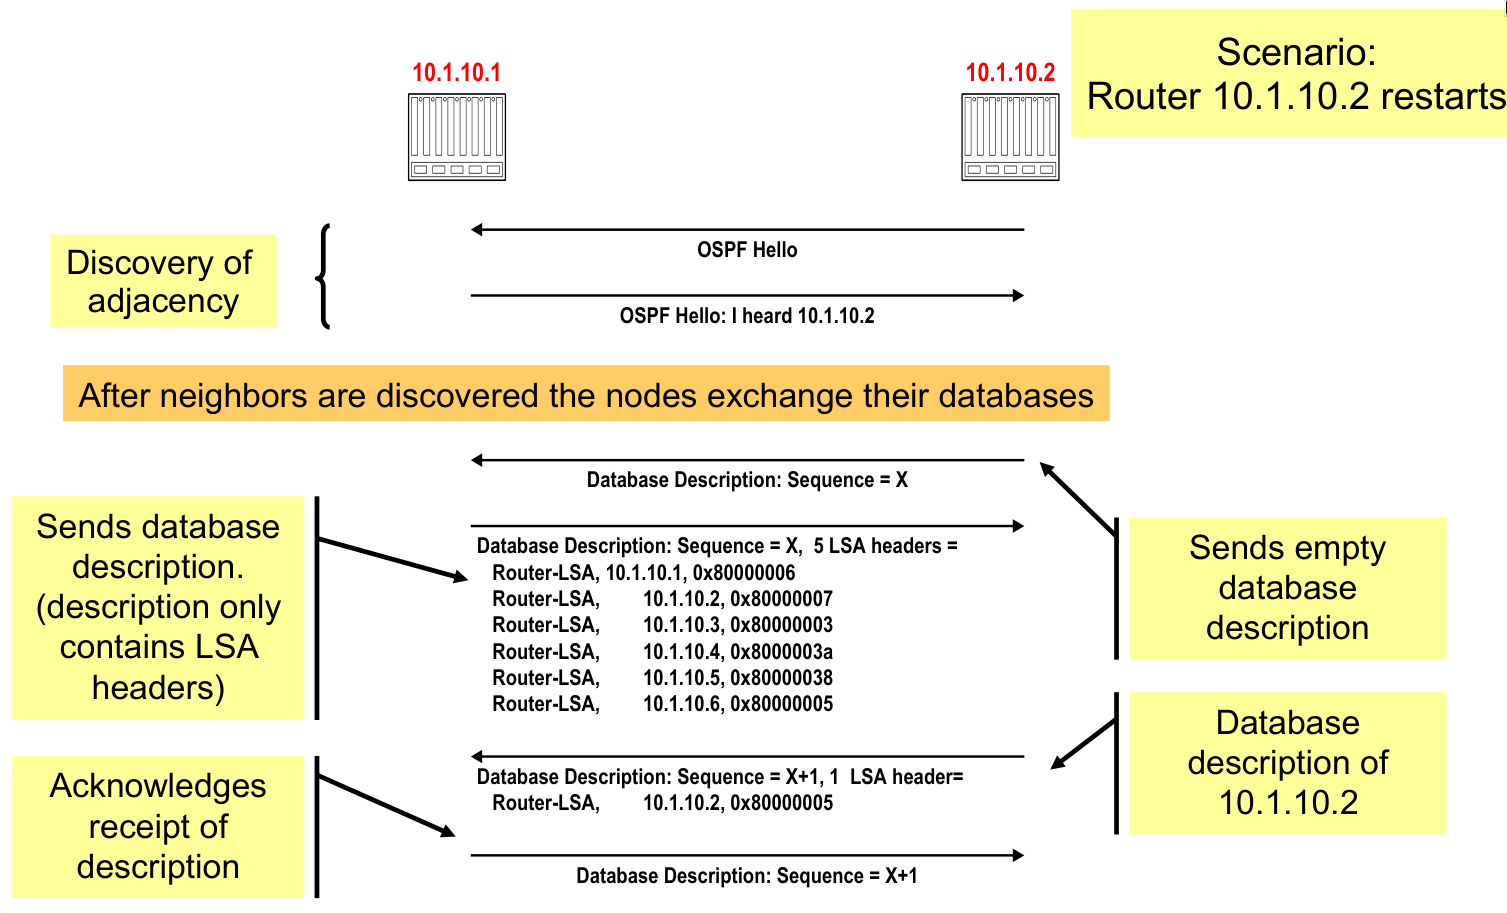
\includegraphics[width=0.8\textwidth]{./images/neighbour_discovery_and_database_synchronisation.png}
    \caption{Neighbours Discovery \& Database Synchronisation}
\end{figure}

\subsection{Regular LSA Exchanges}
\begin{figure}[H]
    \centering
    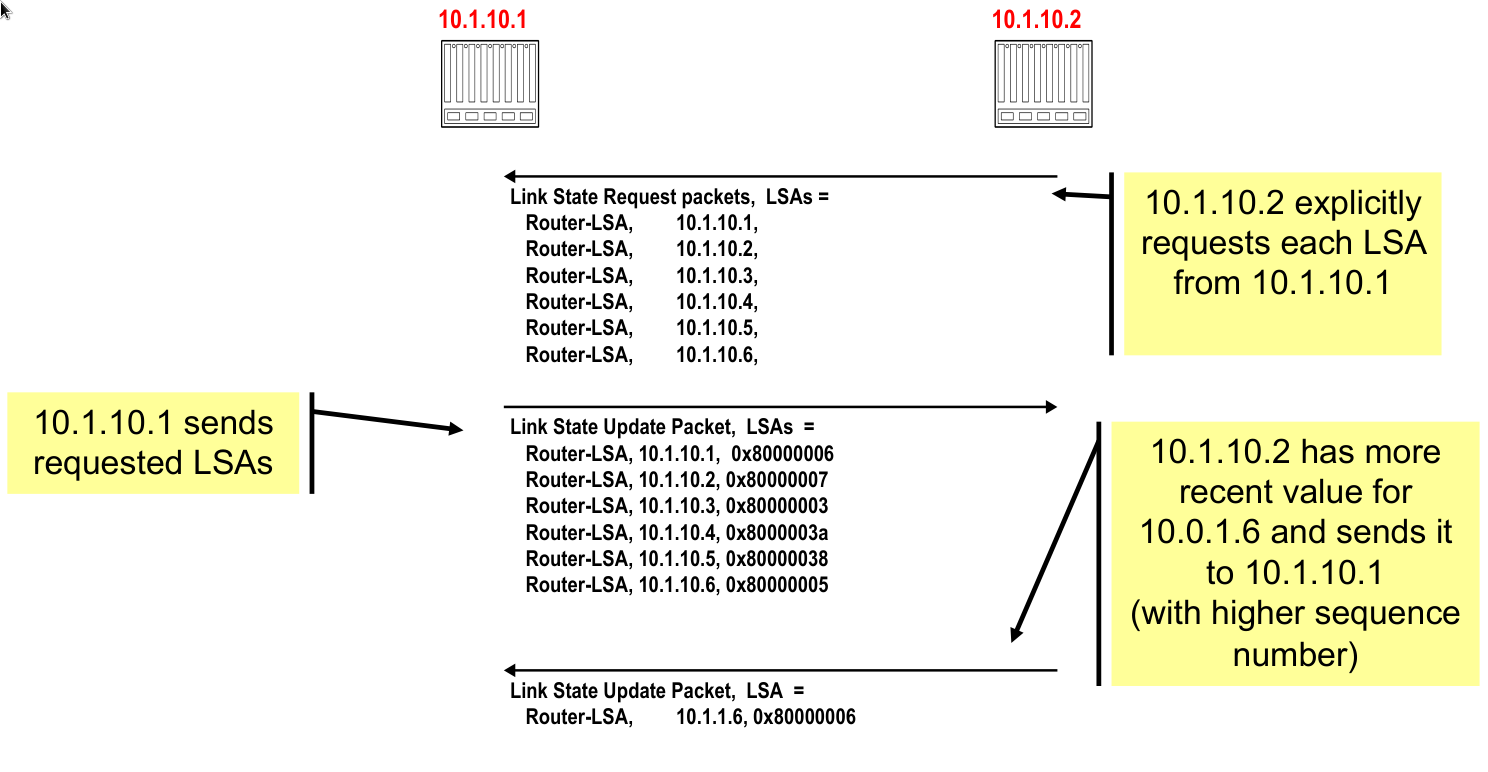
\includegraphics[width=0.8\textwidth]{./images/regular_lsa_exchanges.png}
    \caption{Regular LSA Exchanges}
\end{figure}

\subsection{Routing Data Distribution}
LSA-Updates are distributed to all other routers via \textbf{reliable flooding}.
\begin{figure}[H]
    \centering
    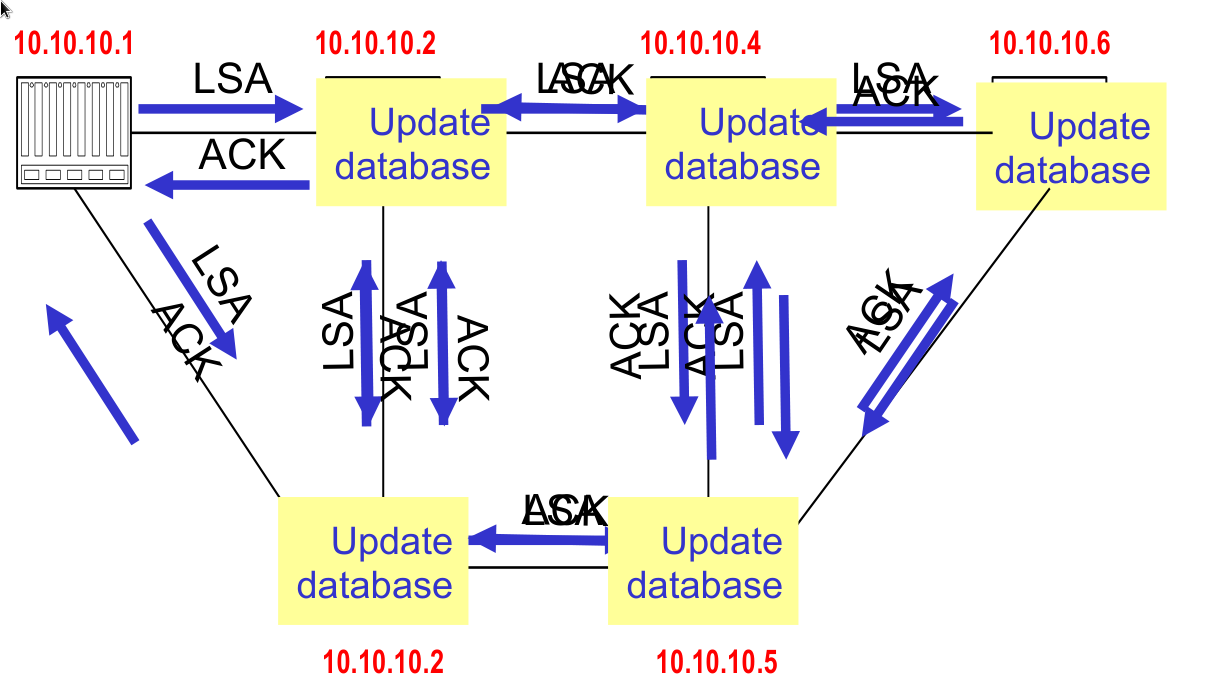
\includegraphics[width=0.8\textwidth]{./images/routing_data_distribution.png}
    \caption{Example: flooding of LSA from \texttt{10.10.10.1}}
\end{figure}

\subsection{Dissemination of LSA-Update}
A router sends and refloods LSA-Updates whenever the topology changes or link costs change.
If a received LSA does not contain new information, the router will not flood the packet.
There is one exception: infrequently (every 30 minutes), a router will flood LSAs even if there are not new changes.
Acknowledgements of LSA-Updates can be explicit with an \verb|ACK| or implicit via reception of an LSA-Update.
\\\\
Once a router has accumulated a full set of link state packets, it can construct the entire subnet graph because every 
link is represented. 
Dijkstra's algorithm will be installed in the routing tables and the normal operation resumed.
\\\\
Practical consideration: for a subnet having $n$ routers, with $k$ neighbours, the memory required to store the input 
data is proportional to $kn$, which may be a problem for large subnets.
Computation time can also be a problem.
In many practical situations, the link state algorithm works well.

\subsection{Hierarchical Routing}
As networks grow in size, the routers' routing tables grow proportionally. 
More CPU time is also required to scan the routing tables, and more bandwidth is required to send new status reports.
At a point, the network may grow so large that it is no longer feasible for every router to have an entry for every
other router, so the routing has to be done hierarchically.
\\\\
The routers are divided into ``\textbf{regions}'', with each router knowing details only about routers in its own region, 
and knowing no details about the internal structures of other regions.
For huge networks, it may be necessary to group the regions into clusters, the clusters into zones, the zones into groups,
an so on, until we run out of names for aggregations.

\begin{figure}[H]
    \centering
    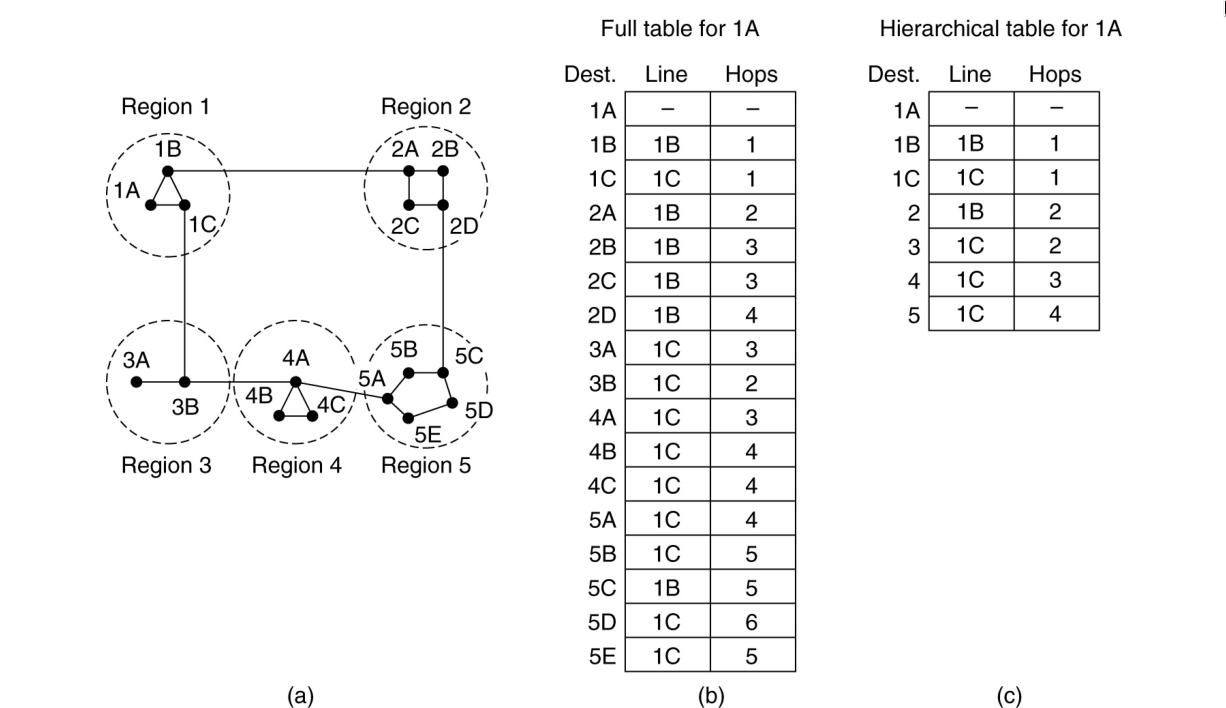
\includegraphics[width=0.8\textwidth]{./images/hierarchical_routing.png}
    \caption{Hierarchical Routing Example}
\end{figure}
 
The above diagram shows routing in a two-level hierarchy with five regions.
The full routing table for 1A has 17 entries.
For hierarchical routing, the routing table has 7 entries.
There is a penalty to be paid in the form of increased path length: the best route from 1A to 5c is through region 2. 
With hierarchical routing, the traffic for region 5 goes through region 3, because that is for most destinations in 
region 5.

\subsubsection{Autonomous Systems}
An \textbf{anonymous system} is a region of the Internet tat is administered by a single entity. 
Examples of autonomous regions include Heanet's national network, Eircom's backbone network, \& Region Internet Service 
Provider.
Routing is done differently within autonomous systems (\textbf{intradomain routing}) and between autonomous systems 
(\textbf{interdomain routing}).

\subsubsection{Border Gateway Protocol (BGP)}
The \textbf{Border Gateway Protocol (BGP)} is an interdomain routing protocol for routing between autonomous systems. 
BGP is currently in version 4. 
It uses TCP to send routing messages. 
BGP is neither a link state nor a distance vector protocol. 
Routing messages in BGP contain complete routes.
Network administrators can specify routing policies.
Note that in the context of BGP, a gateway is nothing other than an IP router that connects autonomous systems.
\\\\
BGP's goal is to find \emph{any} path, not necessarily an optimal one. 
Since the internals of the autonomous system are never revealed, finding an optimal path is not feasible.
For each autonomous system (AS), BGP distinguishes: 
\begin{itemize}
    \item   \textbf{Local traffic:} traffic with a source or destination in the AS.
    \item   \textbf{Transit traffic:} traffic that passes through the AS.
    \item   \textbf{Stub AS:} has connection to only one AS, carries local traffic.
    \item   \textbf{Multihomed AS:} has connections to more than one AS, but does not carry transit traffic.
    \item   \textbf{Transit AS:} has connections to more than one AS, and does carry transit traffic.
\end{itemize}






\end{document}
